% Modelo de slides para projetos de disciplinas do Abel
\documentclass[10pt]{beamer}

\usetheme[progressbar=frametitle]{metropolis}
\usepackage{appendixnumberbeamer}
\usepackage[sort&compress]{natbib}
\bibliographystyle{abbrvnat}

\usepackage{booktabs}
\usepackage[scale=2]{ccicons}

\usepackage{xspace}
\newcommand{\themename}{\textbf{\textsc{metropolis}}\xspace}

\usepackage{algorithmic}
\usepackage{gensymb}

\usepackage[font=scriptsize]{caption}

\setlength{\leftmargini}{1em}

\usepackage{xcolor}
\usepackage{listings, lstautogobble}
\lstset{
    basicstyle=\tiny\ttfamily,
    autogobble=true, 
}

\newcommand{\semitransp}[2][35]{\color{fg!#1}#2}

\title{Group Meeting: Developing some intuition for GEOS-Chem}
% \subtitle{Subtítulo}
% \date{\today}
\date{2019-11-12}
\author{Liam Bindle}
% \institute{UFPR - Disciplina - Semestre}
% \titlegraphic{\hfill\includegraphics[height=1.5cm]{logo.pdf}}

\newcommand{\gccpseudocode}{%
    \small
    \setlength{\tabcolsep}{20pt}
    \begin{table}[]
    \begin{tabular}{ll}
    \hline
    \textbf{GEOS-Chem Classic} & \textbf{main.F lineno}* \\ \hline
    $time \leftarrow starttime$ &  \\
    $S \leftarrow \text{\textbf{READ} restart file}$ &  700 \\
    \textbf{while} $time \neq endtime$ \textbf{do} & 870 \\
    $\quad time \leftarrow time + \Delta t$ & 878 \\
    $\quad \text{\textbf{READ} metfields and emissions}$ & 962 \\
    $\quad M \leftarrow \text{COMPUTE metfield interpolation}$ & 1172 \\
    $\quad S \leftarrow ADVECTION(S, M, \Delta t)$ & 1407 \\
    $\quad S \leftarrow DRY\_DEP(S, M, \Delta t)$ & 1517 \\
    $\quad S \leftarrow EMISSIONS(S, M, \Delta t)$ & 1556 \\
    $\quad S \leftarrow TURB\_MIXING(S, M, \Delta t)$ & 1606 \\
    $\quad S \leftarrow CONVECTION(S, M, \Delta t)$ & 1633 \\
    $\quad S \leftarrow CHEMISTRY(S, M, \Delta t)$& 1691 \\
    $\quad S \leftarrow WET\_DEP(S, M, \Delta t)$ & 1719 \\
    $\quad \text{\textbf{SAVE} diagnostics}$ & 1873-2262 \\
    \textbf{end while} & 2923 \\ \hline
    \multicolumn{2}{r}{\fontsize{4}{4}\selectfont\textit{*GEOS-Chem 12.6.1}} \\
    \end{tabular}
    \end{table}
}

\begin{document}

\maketitle

\begin{frame}{Table of contents}
  \setbeamertemplate{section in toc}[sections numbered]
  \setbeamertemplate{subsection in toc}[circle]
  \tableofcontents
\end{frame}

\section{What does GEOS-Chem actually do?}
\subsection{Realizing the theory}

\begin{frame}[fragile]{Realizing the theory: the continuity equation}
    First, remember the one-box model
    \begin{figure}
        \centering
        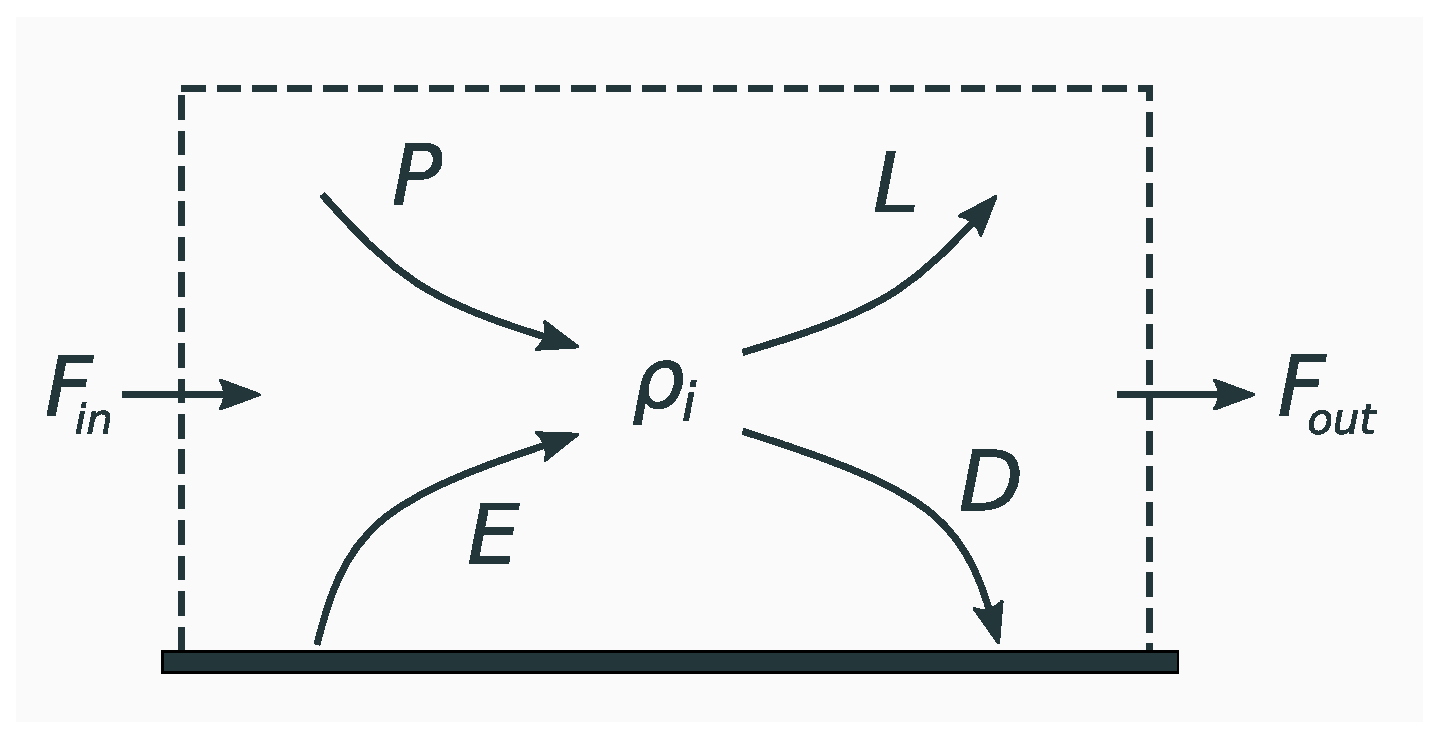
\includegraphics[width=0.5\textwidth]{box-model.eps}
        \captionsetup{labelformat=empty}
        \caption{Adapted from \cite{jacob_introduction_1999}}
    \end{figure}
    \pause
    More generally, CTMs solve the continuity equation
    $$
        \frac{\partial \rho_i}{\partial t} + \boldsymbol \nabla \cdot (\rho_i \boldsymbol v) = s_i
    $$
    \pause
    How does that help?
\end{frame}

\begin{frame}[fragile]{Realizing the theory: the time integral}
    The CTM's goal is to evaluate
    $$
        \rho_i(x, y, z, t) = \rho_i(x, y, z, t_0) + \int_{t_0}^{t} \frac{\partial \rho_i}{\partial t} dt
    $$
    \pause
    \vfill
    which can be written as the sum of timesteps
    \small
    $$
        \rho_i(x, y, z, t_F) = \rho_i(x, y, z, t_0) + \int\displaylimits_{t_0}^{t_0 + \Delta t} \frac{\partial \rho_i}{\partial t} dt  + \int\displaylimits_{t_0 + \Delta t}^{t_0 + 2 \Delta t} \frac{\partial \rho_i}{\partial t} dt + \ldots + \int\displaylimits_{t_F - \Delta t}^{t_F} \frac{\partial \rho_i}{\partial t} dt
    $$
\end{frame}

\begin{frame}[fragile]{Realizing the theory: a timestep}
    A timestep in the time-integral of the continuity equation is
    $$\int_{\Delta t} \frac{\partial \rho_i}{\partial t} dt$$
    Recall the continuity equation
    $$
        \frac{\partial \rho_i}{\partial t} =   \quad \color{blue} -\boldsymbol \nabla \cdot (\rho_i \boldsymbol v) \quad \color{red} + \quad s_i
    $$
    \pause
    \normalsize
    The integrand can be rewritten as
    \tiny
    $$
        \frac{\partial \rho_i}{\partial t} = 
        \color{blue}
        \left[ \frac{\partial \rho_i}{\partial t} \right]_{adv} + 
        \left[ \frac{\partial \rho_i}{\partial t} \right]_{mix} + 
        \left[ \frac{\partial \rho_i}{\partial t} \right]_{conv} \color{red} + 
        \left[ \frac{\partial \rho_i}{\partial t} \right]_{scav} + 
        \left[ \frac{\partial \rho_i}{\partial t} \right]_{chem} + 
        \left[ \frac{\partial \rho_i}{\partial t} \right]_{em} + 
        \left[ \frac{\partial \rho_i}{\partial t} \right]_{dep}
    $$
    \pause
    \normalsize
    So a timestep is
    \tiny
    \begin{align*}
        \int_{\Delta t}\frac{\partial \rho_i}{\partial t} dt = 
        \int_{\Delta t}\left[ \frac{\partial \rho_i}{\partial t} \right]_{adv} dt 
        & + \int_{\Delta t}\left[ \frac{\partial \rho_i}{\partial t} \right]_{mix} dt + 
        \int_{\Delta t}\left[ \frac{\partial \rho_i}{\partial t} \right]_{conv} dt +
        \int_{\Delta t}\left[ \frac{\partial \rho_i}{\partial t} \right]_{scav} dt \\ 
        & + \int_{\Delta t}\left[ \frac{\partial \rho_i}{\partial t} \right]_{chem} dt + 
        \int_{\Delta t}\left[ \frac{\partial \rho_i}{\partial t} \right]_{em} dt + 
        \int_{\Delta t}\left[ \frac{\partial \rho_i}{\partial t} \right]_{dep} dt
    \end{align*}
\end{frame}

\begin{frame}[fragile]{Realizing the theory: GEOS-Chem as an expression}
    \small
    \begin{align*}
        \rho_i(x, y, z, t_F) = \rho_i(x, y, z, t_0) + \sum_{\Delta t \in T} (
        & \int_{\Delta t}\left[ \frac{\partial \rho_i}{\partial t} \right]_{adv} dt \\& + 
        \int_{\Delta t}\left[ \frac{\partial \rho_i}{\partial t} \right]_{dep} dt \\ & + 
        \int_{\Delta t}\left[ \frac{\partial \rho_i}{\partial t} \right]_{em} dt \\& +
        \int_{\Delta t}\left[ \frac{\partial \rho_i}{\partial t} \right]_{mix} dt \\ & + 
        \int_{\Delta t}\left[ \frac{\partial \rho_i}{\partial t} \right]_{conv} dt \\& +
        \int_{\Delta t}\left[ \frac{\partial \rho_i}{\partial t} \right]_{chem} dt \\ & + 
        \int_{\Delta t}\left[ \frac{\partial \rho_i}{\partial t} \right]_{scav} dt )
    \end{align*}
\end{frame}

\begin{frame}[fragile]{GEOS-Chem Classic in pseudocode}
    \gccpseudocode
\end{frame}

\subsection{Transport term processes}
\frame{\sectionpage}

\begin{frame}[fragile]{Transport term processes: advection}
    \begin{minipage}[c]{0.5\textwidth}
        \begin{itemize}
            \item Transport of tracers by wind
            \vspace{0.3cm}
            \item GEOS-Chem uses the \textbf{TPCORE} and \textbf{FV3} advection algorithms
        \end{itemize}
            \vspace{0.5cm}
            \textbf{Input} 
            \begin{itemize}
                \item Tracer mixing ratios
                \item Meteorological variables
            \end{itemize}
            \textbf{Output}
            \begin{itemize}
                \item Mixing ratios after $\Delta t$
            \end{itemize}
    \end{minipage} \hfill
    \begin{minipage}[c]{0.49\textwidth}
    \begin{center}
        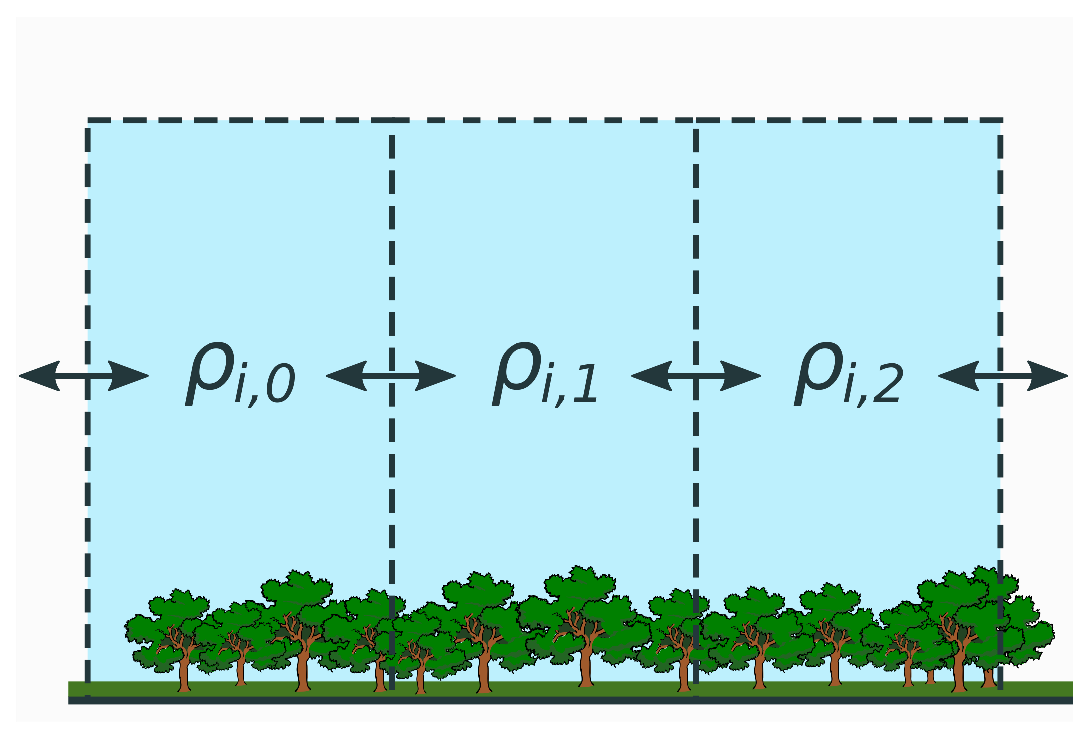
\includegraphics[width=0.9\textwidth]{box-model-advection.eps}    
    \end{center}
    \vspace{0.5cm}
    $$
        \left[ \frac{\partial \rho_i}{\partial t} \right]_{adv} + \boldsymbol \nabla \cdot (\rho_i \boldsymbol v) = 0
    $$
    \end{minipage}
\end{frame}

\begin{frame}[fragile]{Transport term processes: mixing}
    \begin{minipage}[c]{0.39\textwidth}
        \begin{center}
            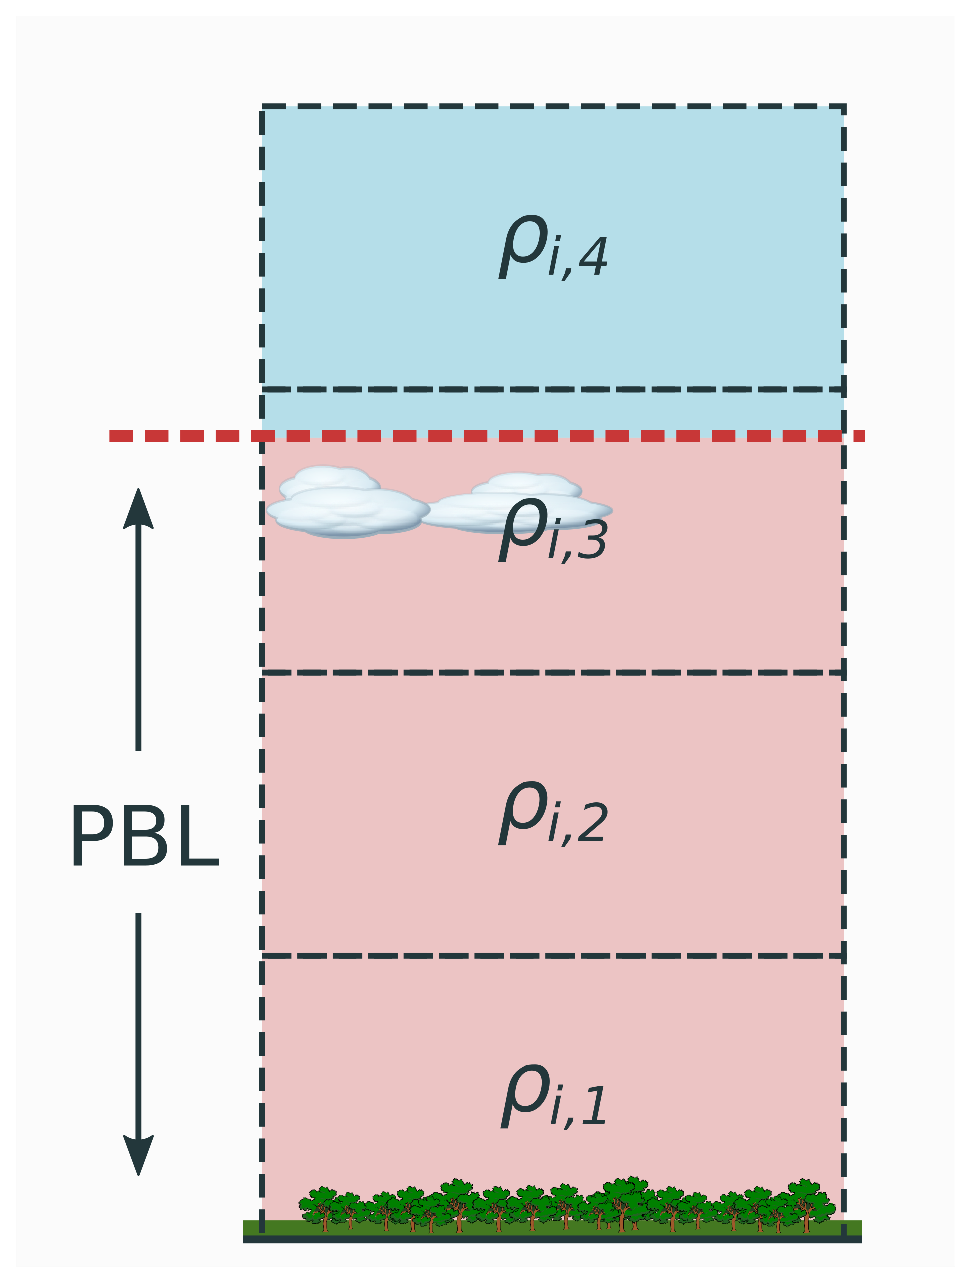
\includegraphics[width=0.9\textwidth]{box-model-mixing.eps}
        \end{center}
        \vspace{5mm}
        \footnotesize
        $$
            \left[ \frac{\partial \rho_i}{\partial t} \right]_{mix} = -\frac{\partial}{\partial z} \left[-K_z \left(\frac{\partial \mu_i}{\partial z} - \gamma_c \right)\right]
        $$
    \end{minipage} \hfill
    \begin{minipage}[c]{0.6\textwidth}
        \small
        \begin{itemize}
            \item Contributes to vertical transport in the PBL
            \item Flux is proportional to concentration gradient
        \end{itemize}
        \vspace{0.5cm}
        Two PBL mixing schemes are available
        \begin{itemize}
            \item \textbf{TURBDAY}: Full PBL mixing
            \item \textbf{VDIFF}: Non-local PBL mixing
            \item User configures PBL mixing in \texttt{input.geos}
            \begin{verbatim}
  Turn on PBL Mixing?    : T
  => Use non-local PBL?  : F
            \end{verbatim}
        \end{itemize}
    \end{minipage}
\end{frame}

\begin{frame}[fragile]{Transport term processes: convection}
    \begin{minipage}[c]{0.5\textwidth}
        \begin{figure}
            \centering
            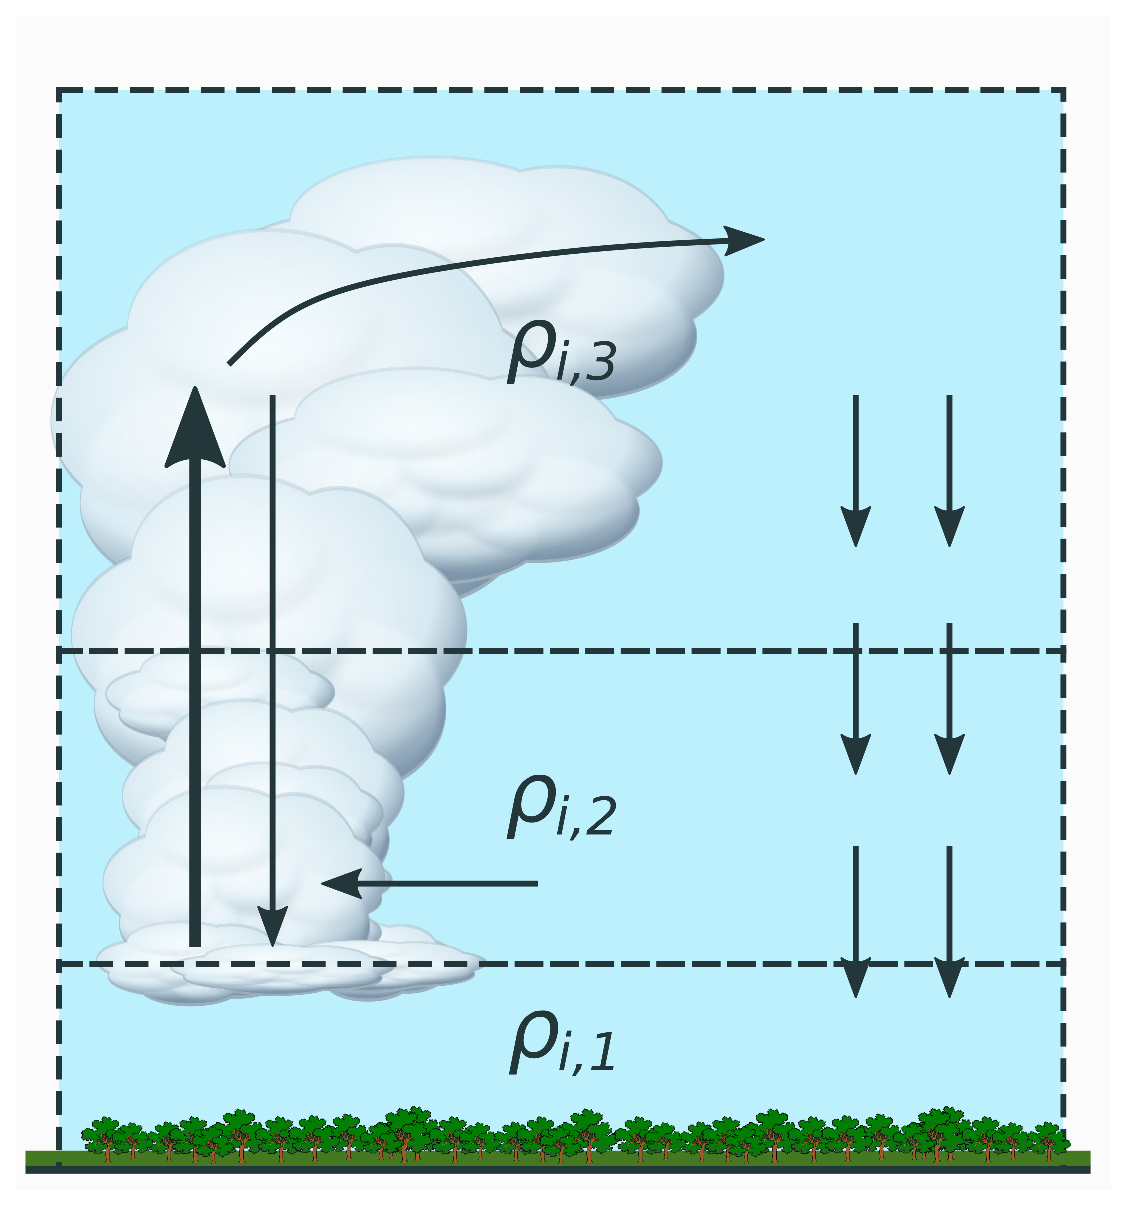
\includegraphics[width=0.9\textwidth]{box-model-convection.eps}
            \captionsetup{labelformat=empty}
            \caption{Adapted from \cite{brasseur_modeling_2017}}
        \end{figure}
    \end{minipage}
    \begin{minipage}[c]{0.49\textwidth}
        \begin{itemize}
            \item Vertical transport
            \vspace{4mm}
            \item GEOS-Chem uses the \textbf{Relaxed Arakawa-Schubert scheme}
            \vspace{4mm}
            \begin{itemize}
                \item Uses convective mass fluxes meteorological archives
            \end{itemize}
            \vspace{4mm}
            \item Entrainment, detrainment, and downdrafts
        \end{itemize}
    \end{minipage}
    $$
        \left[ \frac{\partial \rho_i}{\partial t} \right]_{conv} = - \frac{\partial}{\partial z} \left[M_u (\mu_{i,u} - \mu_{i}) + M_d (\mu_{i,d} - \mu_{i}) \right] 
    $$
\end{frame}

\subsection{Source term processes}
\frame{\sectionpage}

\begin{frame}[fragile]{Source term processes: scavenging}
    \begin{center}
    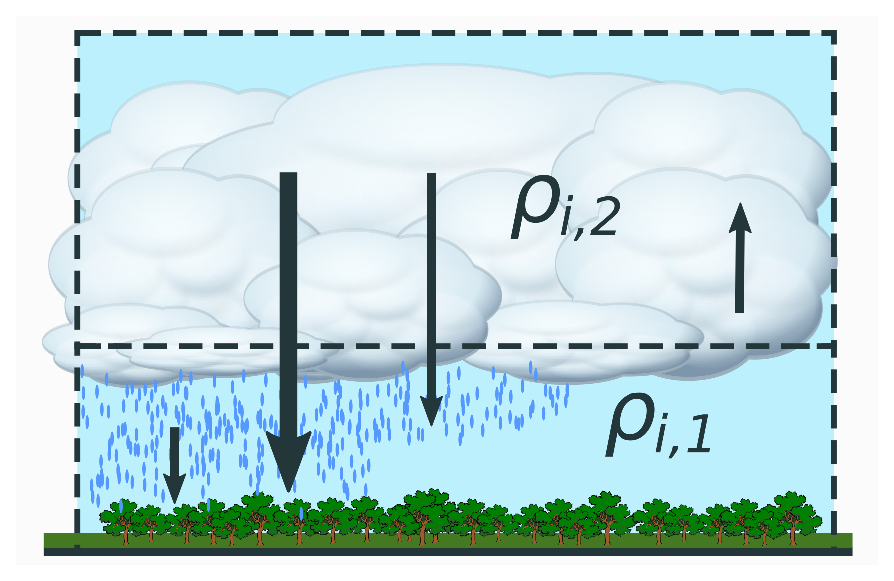
\includegraphics[width=0.5\textwidth]{box-model-scav.eps}
    \end{center}
    \begin{itemize}
        \item Modelled processes include rainout, washout, riming, virga
        \item Scavenging by liquid, solid, and mixed precipitation
        \item Gases and aerosols are scavenged
    \end{itemize}
\end{frame}

\begin{frame}[fragile]{Source term processes: chemistry (1/2)}
    \begin{itemize}
        \item Chemical production and loss of a species is handled by FlexChem (based on KPP)
        \item KPP is a utility that generates Fortran code 
        \begin{itemize}
            \item Generated code evaluates the time integral of a kinetic system
            \item Kinetic system is a system of coupled ODEs
        %    \item Kinetic system is described in an input file(variable species, constant species, %and reactions)
        %    \item GC uses Rosenbrock Integrator
        \end{itemize}
        \vfill
        \begin{figure}
            \centering
            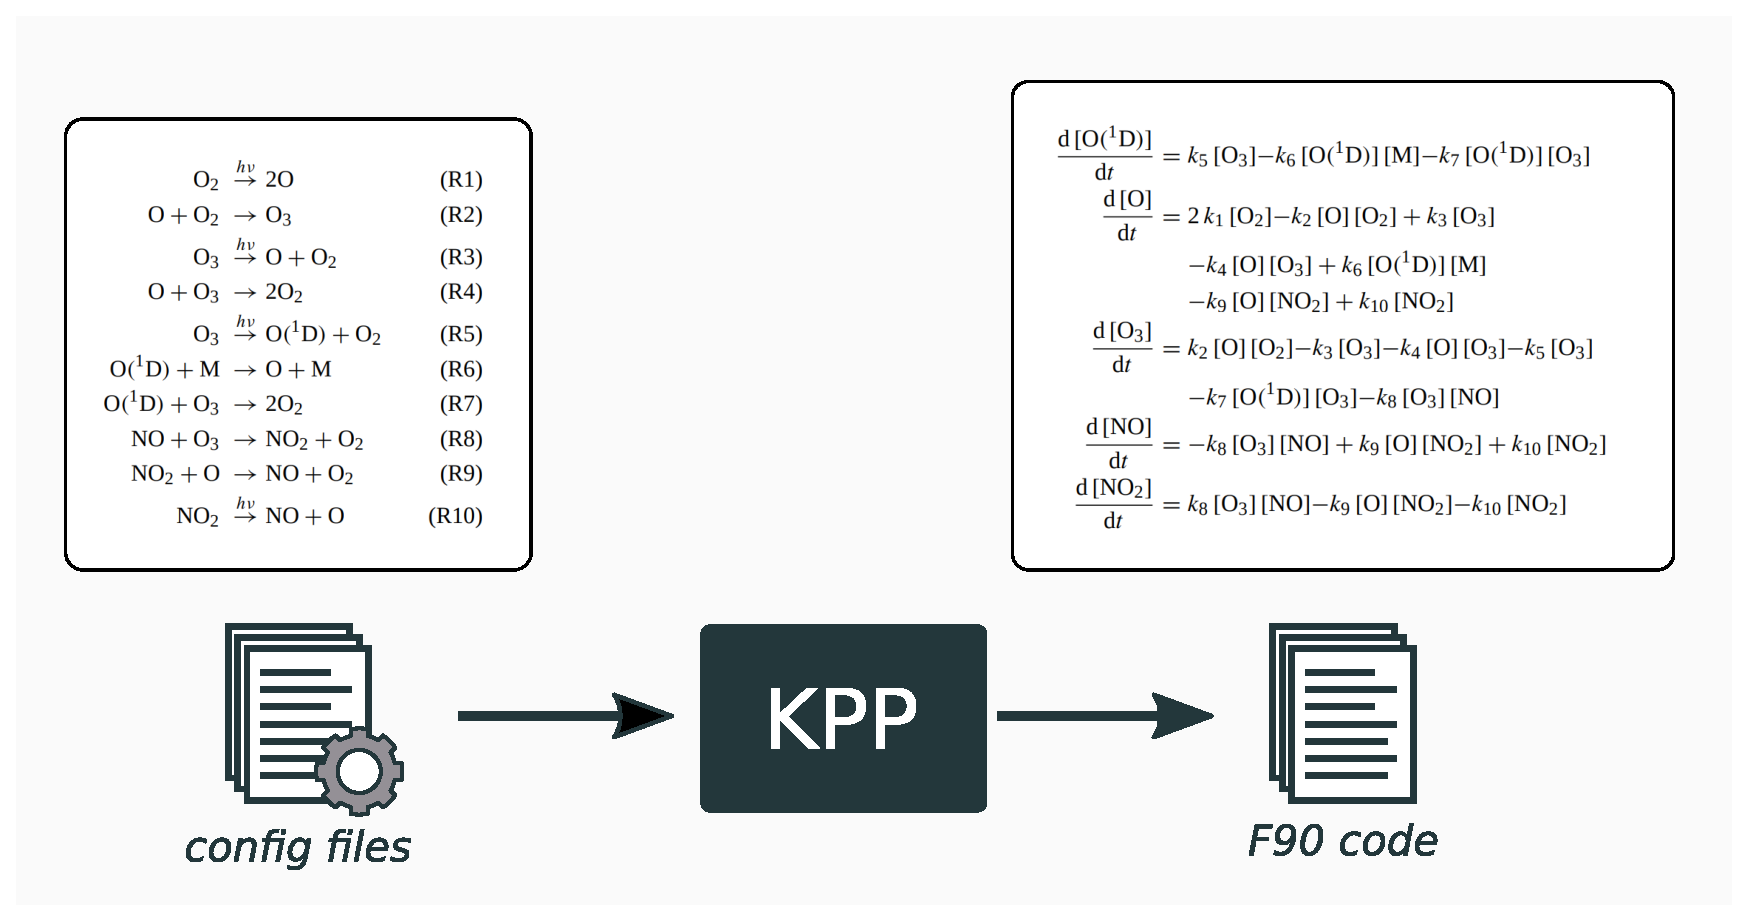
\includegraphics[width=0.7\textwidth]{kpp.eps}
            \captionsetup{labelformat=empty}
            \caption{Adapted from \cite{sandu_technical_2006}}
        \end{figure}
    \end{itemize}
\end{frame}

\begin{frame}[fragile]{Source term processes: chemistry (2/2)}
    GC has three chemical mechanisms to choose from
    
    \small
    \begin{table}[]
    \begin{tabular}{lccl}
        \hline
        \textbf{Mechanism} & \textbf{Species} & \textbf{Reactions} & \textbf{Notes} \\ 
        \hline
        Standard & 243 & 730 & full chemistry + UCX \\ 
        Tropchem & 226 & 650 & full chemistry \\ 
        SOA\_SVPOA & 230 & 653 & full chemistry + complex SOA \\
         & & & and SVPOA chemistry \\ 
        \hline
    \end{tabular}
    \end{table}
    \begin{minipage}[c]{0.6\textwidth}
        \normalsize
        \textbf{Fully chemistry}
        \begin{itemize}
            \item NOx-Ox-HC-Aer-Br-Cl-I kinetic system
        \end{itemize}
        
        \textbf{UCX}
        \begin{itemize}
            \item Combines tropospheric and stratospheric reactions into a single mechanism
        \end{itemize}
    \end{minipage}
    \begin{minipage}[c]{0.34\textwidth}
        $$
            \left[ \frac{\partial \rho_i}{\partial t} \right]_{chem} = P_i - L_i \rho_i
        $$
    \end{minipage}
\end{frame}

\begin{frame}[fragile]{Source term processes: emissions}
    \begin{itemize}
        \item GC uses HEMCO to compute emissions
        \begin{itemize}
            \item Combines emission inventories from many sources into unified emission model
            \item Allows for temporal (e.g. day-of-week) and environmental (e.g. wind, sza, etc.) parameterizations
        \end{itemize}
        \item HEMCO is configured in \texttt{HEMCO\_Config.rc}
        \vfill
    \end{itemize}
    \begin{minipage}[c]{0.7\textwidth}
        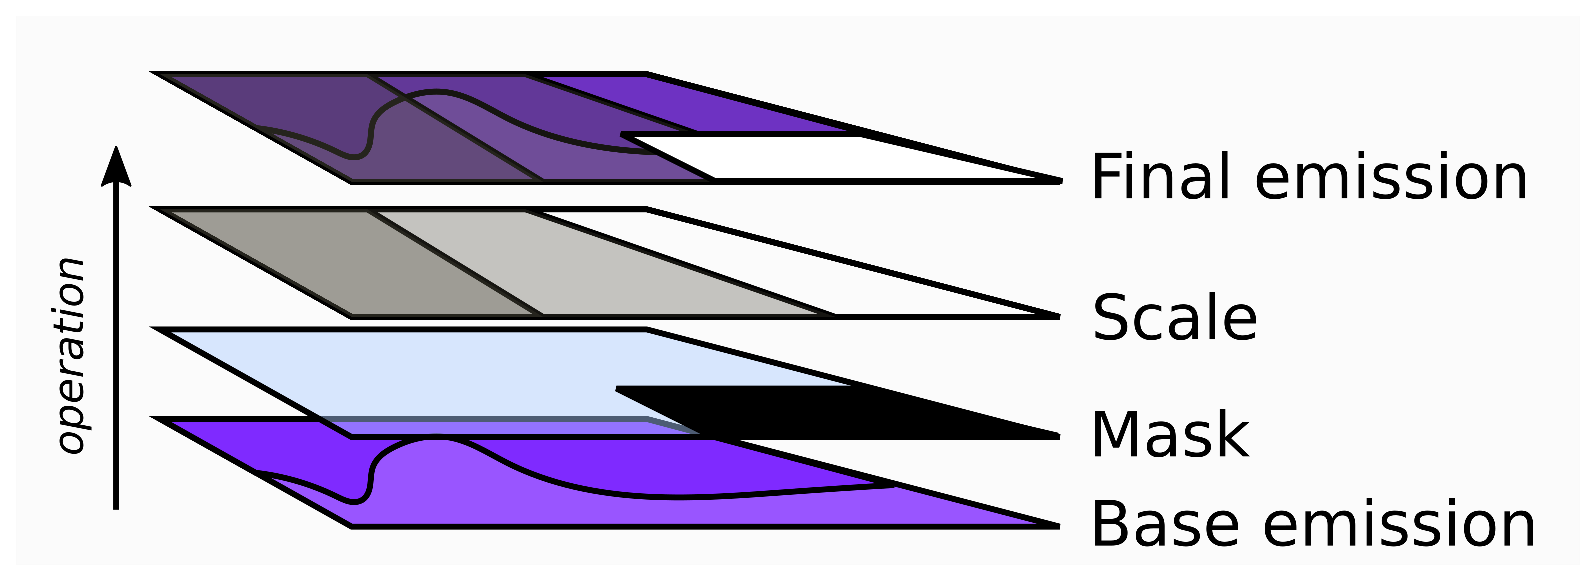
\includegraphics[width=\textwidth]{hemco.eps}
    \end{minipage}
    \begin{minipage}[c]{0.29\textwidth}
        $$
            \left[ \frac{\partial \rho_i}{\partial t} \right]_{em} = \frac{E_i }{\Delta z_1}
        $$
    \end{minipage}
\end{frame}

\begin{frame}[fragile]{Source term processes: deposition}
        \begin{minipage}[c]{0.49\textwidth}
        \small
        \begin{itemize}
            \item \textit{Resistance-in-series} parameterization
            \vspace{0.3cm}
            \item $1/R$ relates deposition rate to conditions and surface
            \vspace{0.3cm}
            \item $R_A$: Turbulent transport surface layer
            \vspace{0.3cm}
            \item $R_{B,i}$: Diffusion through quasi-laminar boundary layer
            \vspace{0.3cm}
            \item $R_{C,i}$: Surface uptake
        \end{itemize}
    \end{minipage} \hfill
    \begin{minipage}[c]{0.5\textwidth}
    \begin{figure}
        \centering
        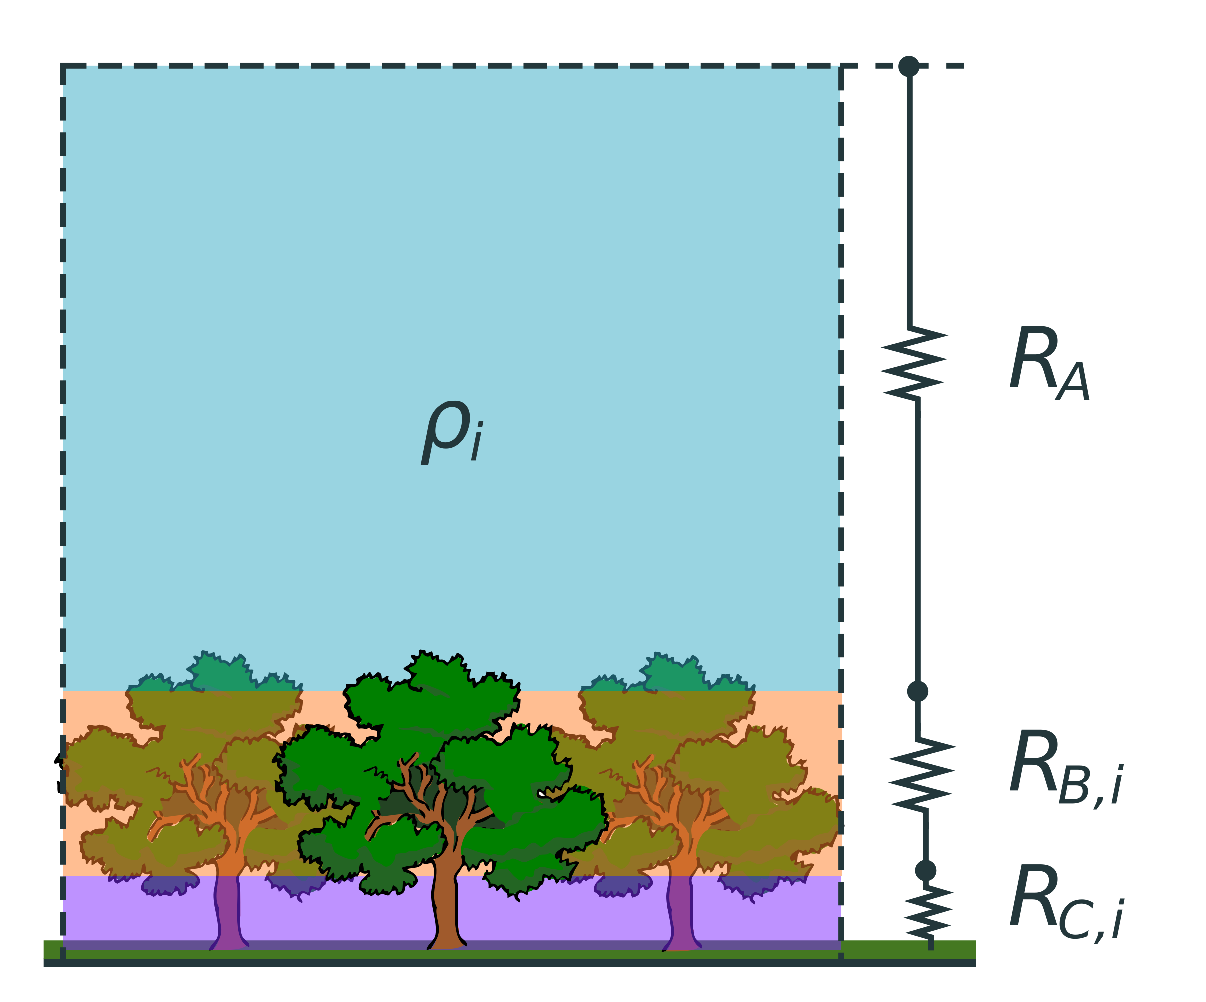
\includegraphics[width=\textwidth]{box-model-dep.eps}    
        \captionsetup{labelformat=empty}
        \caption{Adapted from \cite{brasseur_modeling_2017}}
    \end{figure}
    $$
        w_{D,i} = \frac{1}{R_A + R_{B,i} + R_{C,i}} \quad [\text{cm s}^{-1}]
    $$ 
    \vspace{0.1cm}
    $$
        \left[ \frac{\partial \rho_i}{\partial t} \right]_{dep} = - \frac{w_{D,i}(z_1) \rho_i(z_1)}{\Delta z_1} 
    $$
    \end{minipage}
\end{frame}

\begin{frame}[fragile]{Vertical grid}
    \begin{minipage}[c]{0.5\textwidth}
    \begin{itemize}
        \item Hybrid sigma-pressure grid
        \vspace{3mm}
        \item Bottom level follows Earth's surface
        \vspace{3mm}
        \item TOA at 0.01 hPa (80.6 km)
        \vspace{3mm}
        \item Same vertical grid as met data
        \vspace{3mm}
        \begin{itemize}
            \item GEOS-FP: 72-layers
            \vspace{3mm}
            \item MERRA-2: 47-layers
        \end{itemize}
    \end{itemize}
    \end{minipage}
    \begin{minipage}[c]{0.49\textwidth}
        \begin{figure}
            \centering
            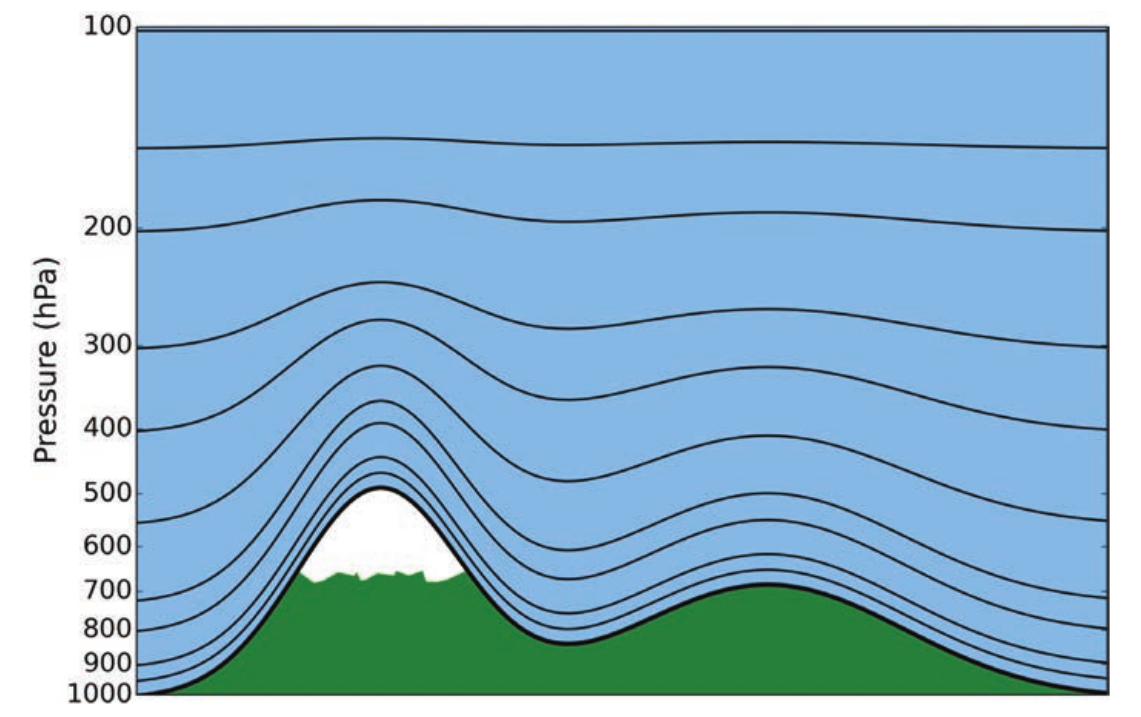
\includegraphics[width=\textwidth]{hybrid-sigma-pressure.png}
            \captionsetup{labelformat=empty}
            \caption{From \cite{brasseur_modeling_2017}}
        \end{figure}
        $$
            p(z_k) = A_k p_0 + B_k p_s
        $$
    \end{minipage}
\end{frame}

\begin{frame}[fragile]{Horizontal grid}
    \small
    \begin{minipage}[c]{0.5\textwidth}
        \begin{table}[]
        \begin{tabular}{lrr}
            \hline
            \multicolumn{3}{l}{\textbf{GEOS-Chem Classic}} \\ 
            Grid & \# boxes & Scale \\ 
            \hline
            4x5$^{\circ}$ & 3,312 & 392 km \\ 
            2x2.5$^{\circ}$ & 13,248 & 196 km \\ 
            \hline
        \end{tabular}
        \end{table}
    \end{minipage}
    \begin{minipage}[c]{0.49\textwidth}
        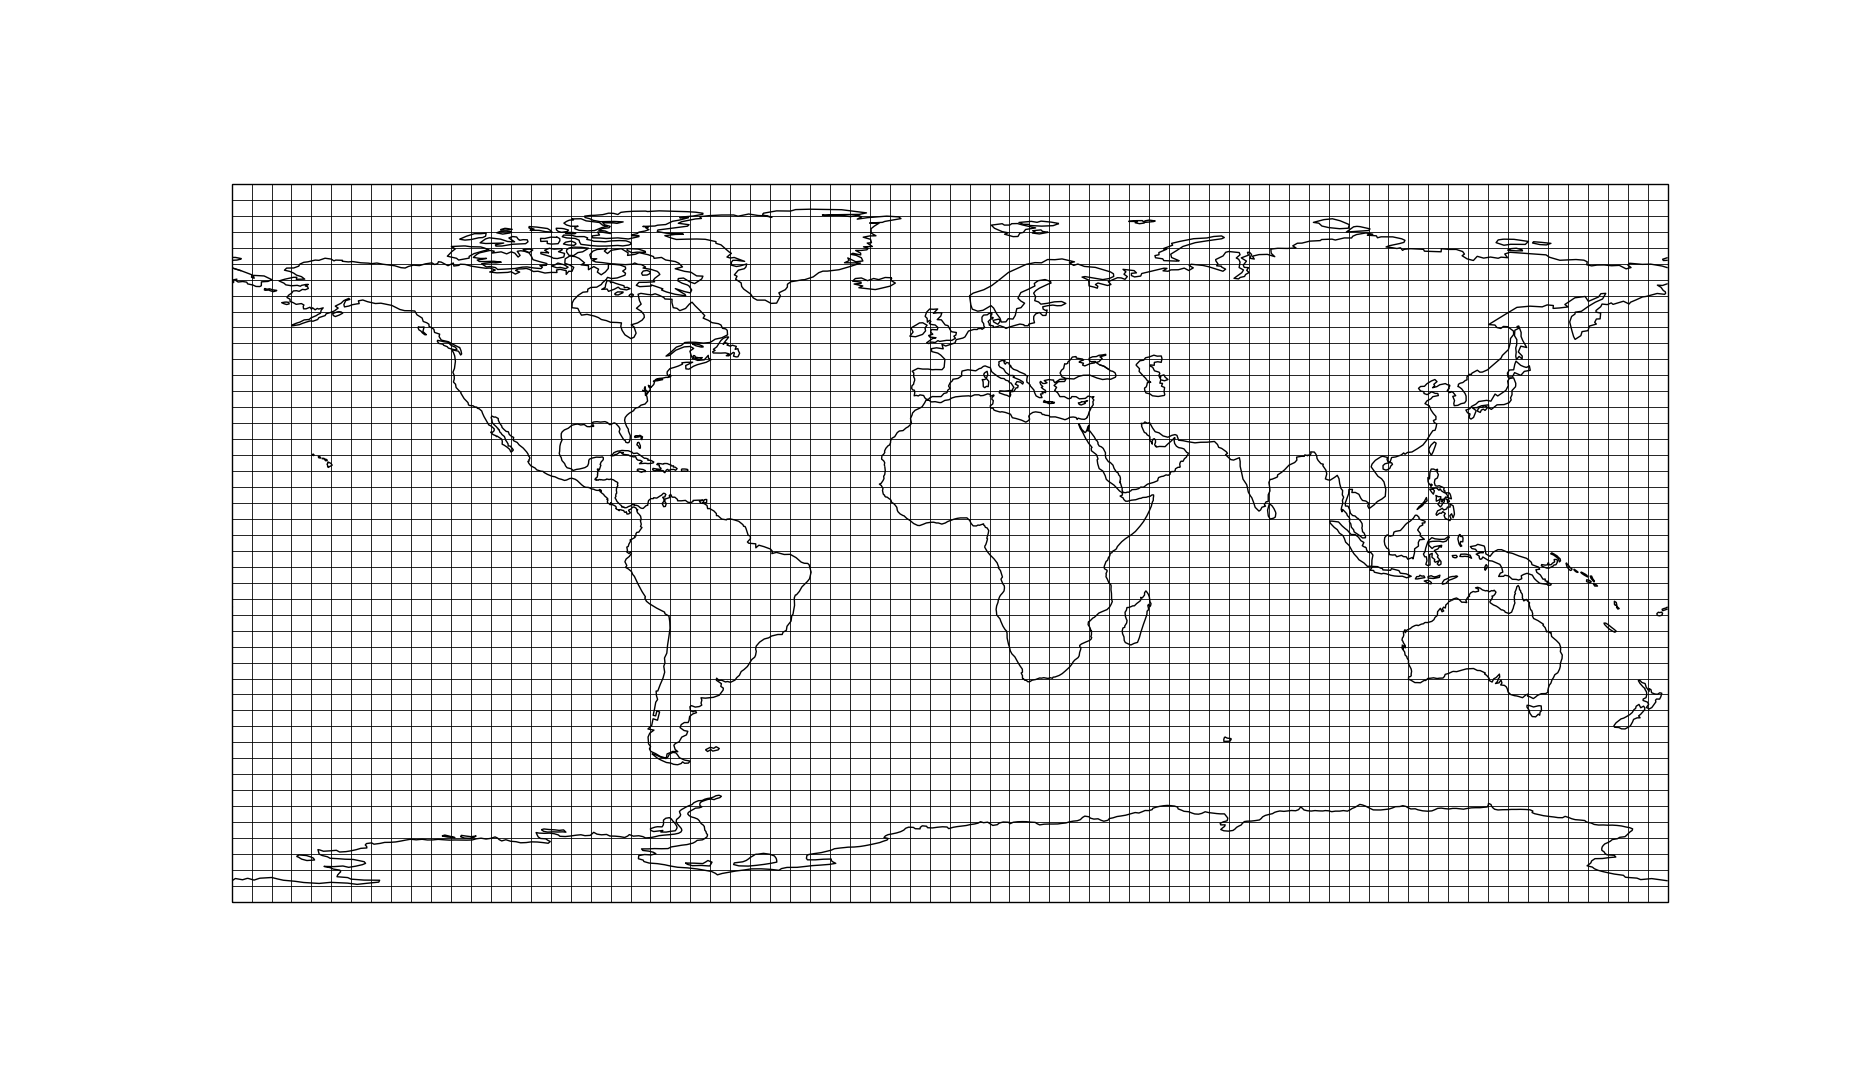
\includegraphics[height=0.4\textheight]{hgrid_4x5.png}
    \end{minipage}

    \small
    \begin{minipage}[c]{0.5\textwidth}
        \begin{table}[]
        \begin{tabular}{lrr}
        \hline
            \multicolumn{3}{l}{\textbf{GCHP}} \\ 
            Grid & \# boxes & Scale \\ 
            \hline
            C24 & 3,456 & 384 km\\ 
            C48 & 13,824 & 192 km\\ 
            C90 & 48,600 & 102 km \\ 
            C180 & 194,400 & 51 km \\ 
            C360 & 777,600 & 26 km \\ 
            \hline
        \end{tabular}
        \end{table}
    \end{minipage}
    \begin{minipage}[c]{0.49\textwidth}
        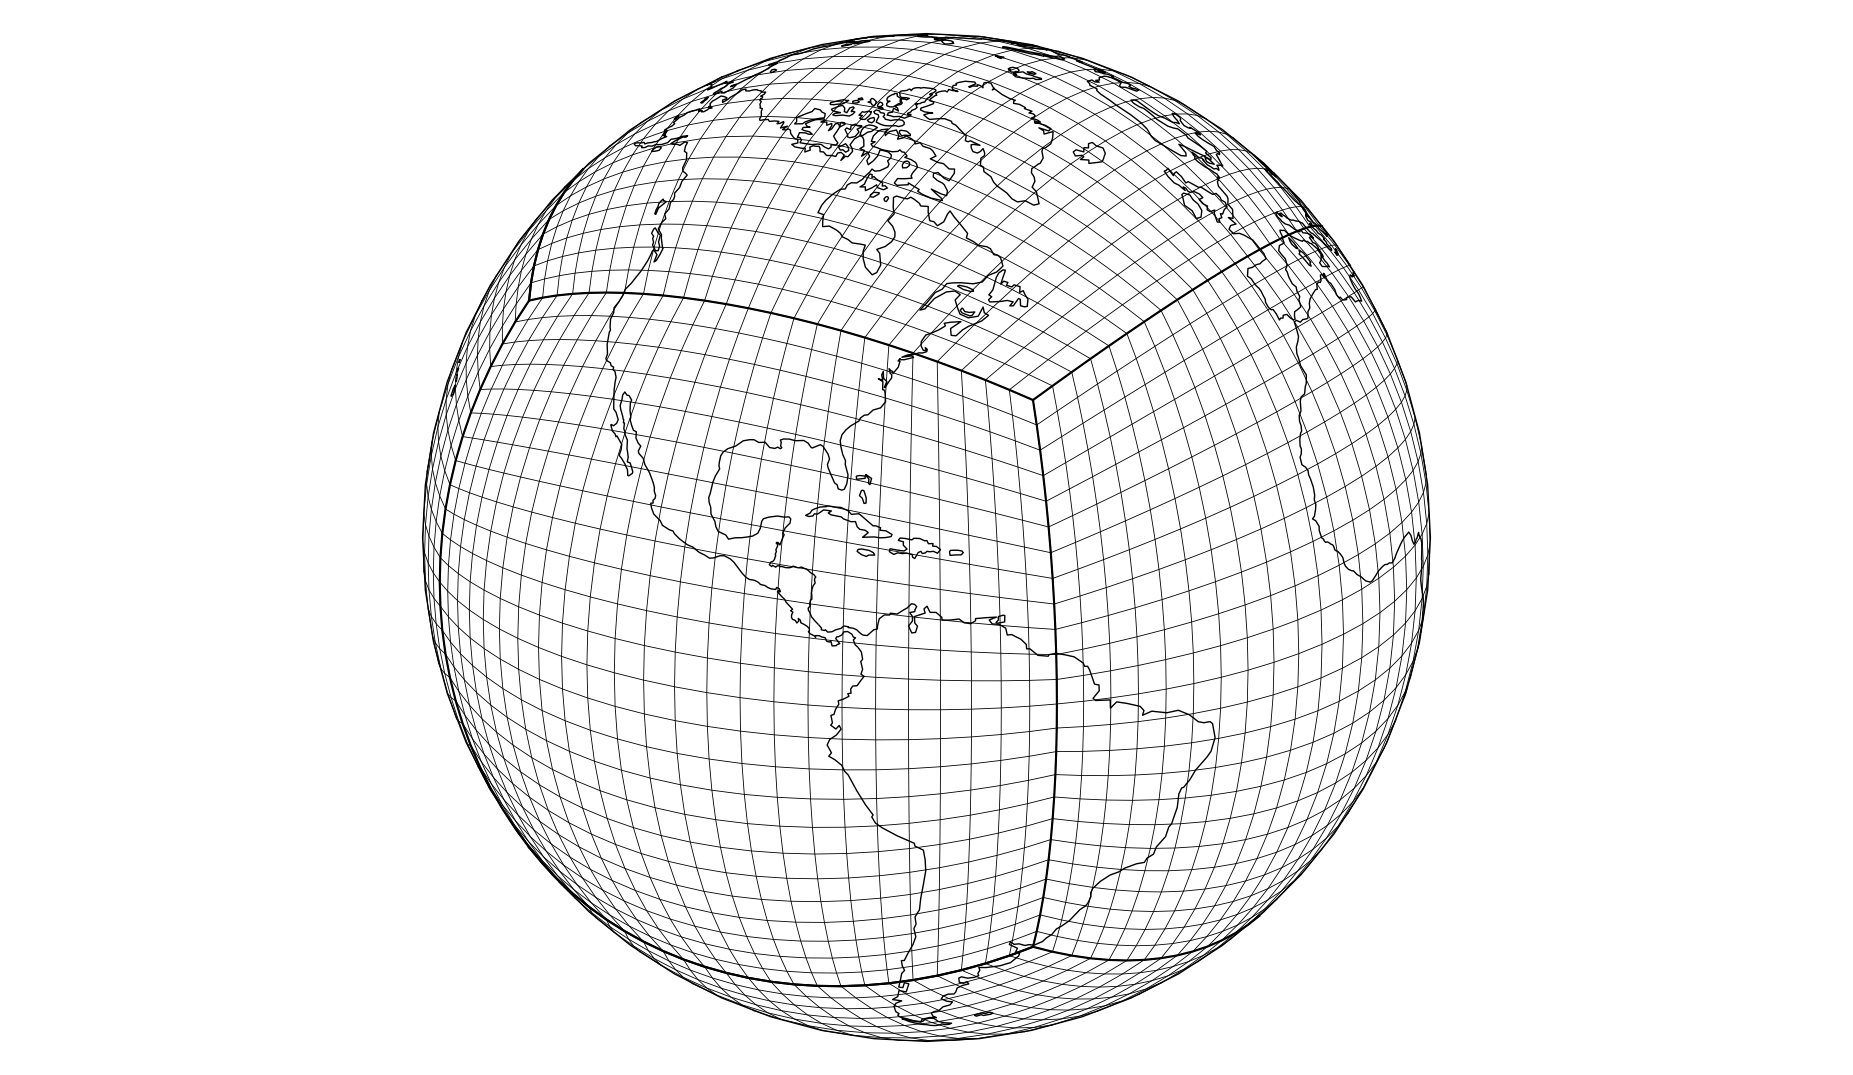
\includegraphics[height=0.4\textheight]{hgrid_c24.png}
    \end{minipage}
\end{frame}

\begin{frame}{GEOS-Chem Classic in pseudocode}
    \vspace{3mm}
    \gccpseudocode
\end{frame}

\section{GCHP and how it's different}

\begin{frame}{GCHP: how's it different?}
    \begin{minipage}[c]{0.39\textwidth}
        \begin{figure}
            \centering
            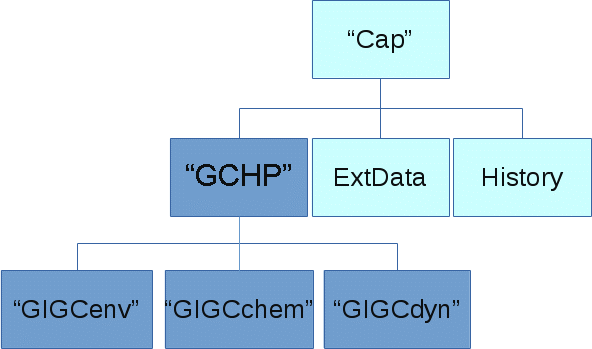
\includegraphics[width=\textwidth]{gchp_components.png}
            \captionsetup{labelformat=empty}
            \caption{From \cite{geos-chem_developers_developing_2019}}
        \end{figure}
    \end{minipage}
    \begin{minipage}[c]{0.6\textwidth}
        \begin{itemize}
            \item GCHP is GEOS-Chem Classic's analog in the MAPL framework
            \vspace{3mm}
            \item MAPL is for \textit{compartmentalizing} and \textit{coupling} Earth systems models 
            \vspace{3mm}
            \begin{itemize}
                \item Models are broken up into \textit{components}
                \vspace{3mm}
                \item Each component has a set of input and outputs
                \vspace{3mm}
                \item Components are automatically interconnected
                \vspace{3mm}
                \item Supports distributed computing
            \end{itemize}
        \end{itemize}
    \end{minipage}
\end{frame}

\begin{frame}[fragile]{GCHP in pseudocode}

    \scriptsize
    \setlength{\tabcolsep}{20pt}
    \begin{table}[]
    \begin{tabular}{ll}
    \hline
    \textbf{Grid-Independent GEOS-Chem (``GIGCchem'')} & \textbf{gigc\_chunk\_mod.F90 lineno}* \\ \hline
    \textbf{FUNCTION}   GIGC\_Chunk\_Run & 369 \\
    $\quad \textbf{INPUT}\ S, M, \Delta t$ &  \\
    $\quad \textbf{OUTPUT}\ S $ & \\
    $\quad S \leftarrow CONVECTION(S, M, \Delta t)$ & 824 \\
    $\quad S \leftarrow DRY\_DEP(S, M, \Delta t)$ & 845 \\
    $\quad S \leftarrow EMISSIONS(S, M, \Delta t)$ & 875 \\
    $\quad S \leftarrow TURB\_MIXING(S, M, \Delta t)$ & 941 \\
    $\quad S \leftarrow CHEMISTRY(S, M, \Delta t)$& 994 \\
    $\quad S \leftarrow WET\_DEP(S, M, \Delta t)$ & 1020 \\
    
    \textbf{END FUNCTION} & 2923 \\ \hline
    \multicolumn{2}{r}{\fontsize{4}{4}\selectfont\textit{*GEOS-Chem 12.6.1}} \\
    \end{tabular}
    \end{table}
    \footnotesize
    \begin{minipage}[c]{0.6\textwidth}
        \begin{itemize}
            \item Advection is done by GMAO's FV3 (``GIGCdyn'')
            \vspace{0.2cm}
            \item Diagnostics are saved by ``History''
            \vspace{0.2cm}
            \item External data is read-in by ``ExtData''
        \end{itemize}
    \end{minipage}
    \begin{minipage}[c]{0.39\textwidth}
        \begin{figure}
            \centering
            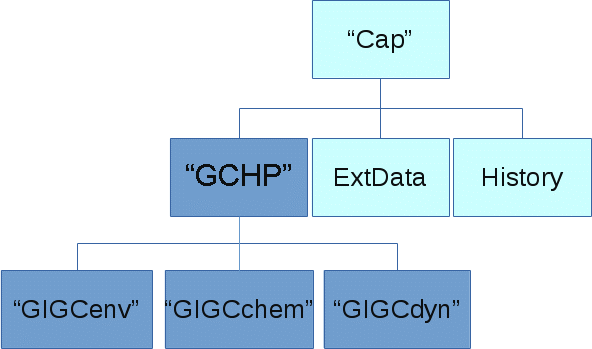
\includegraphics[width=\textwidth]{gchp_components.png}
            \captionsetup{labelformat=empty}
            \caption{From \cite{geos-chem_developers_developing_2019}}
        \end{figure}
    \end{minipage}
    
    % \paragraph{Note: Without overhead, $S$ at C360 is 98 GB (55,987,200 boxes, 218 species, 8 byte float). Saving $S$ after each timestep would result in 7.1 TB of output per simulation day (20 min chemistry timestep; 2.6 PB/year).}
\end{frame}

\begin{frame}[fragile]{GCHP: benefits and challenges }
    \textbf{Benefits}
    \footnotesize
    \begin{itemize}
        \item GCHP can run across multiple nodes
        \item Can leverage other models written in the MAPL framework (e.g. FV3)
        \item Other models can use the GEOS-Chem component (e.g. GEOS-Chem in GEOS)
    \end{itemize}
    \vfill
    \normalsize
    \textbf{Challenges} (outward facing)
    \footnotesize
    \begin{itemize}
        \item MAPL adds a lot of complexity
        \item More things can go wrong
        \item GCHP is harder to build
    \end{itemize}
\end{frame}

\subsection{Making GCHP easier to use}
\frame{\sectionpage}

\begin{frame}[fragile]{Making GCHP easier to build: CMake support}
    \begin{minipage}[c]{0.6\textwidth}
        \footnotesize
        \begin{enumerate}
            \item Navigate to your run directory
            \begin{lstlisting}[language=bash,morekeywords={mkdir,cmake,make},]
            cd ~/geosfp_2x25_standard
            \end{lstlisting}
            \item Create your build directory and \texttt{cd} into it
            \begin{lstlisting}[language=bash,morekeywords={mkdir,cmake,make},]
            ~/geosfp_2x25_standard> mkdir build
            ~/geosfp_2x25_standard> cd build
            \end{lstlisting}
            \item Configure GEOS-Chem's build
            \begin{lstlisting}[language=bash,morekeywords={mkdir,cmake,make},]
            ~/geosfp_2x25_standard/build> cmake /path/to/geos-chem
            \end{lstlisting}
            \item Compile GEOS-Chem
            \begin{lstlisting}[language=bash,morekeywords={mkdir,cmake,make},]
            ~/geosfp_2x25_standard/build> make -j
            \end{lstlisting}
            \item Install \texttt{geos} in run directory
            \begin{lstlisting}[language=bash,morekeywords={mkdir,cmake,make},]
            ~/geosfp_2x25_standard/build> make install
            \end{lstlisting}
        \end{enumerate}

    \end{minipage}
    \begin{minipage}[c]{0.39\textwidth}
        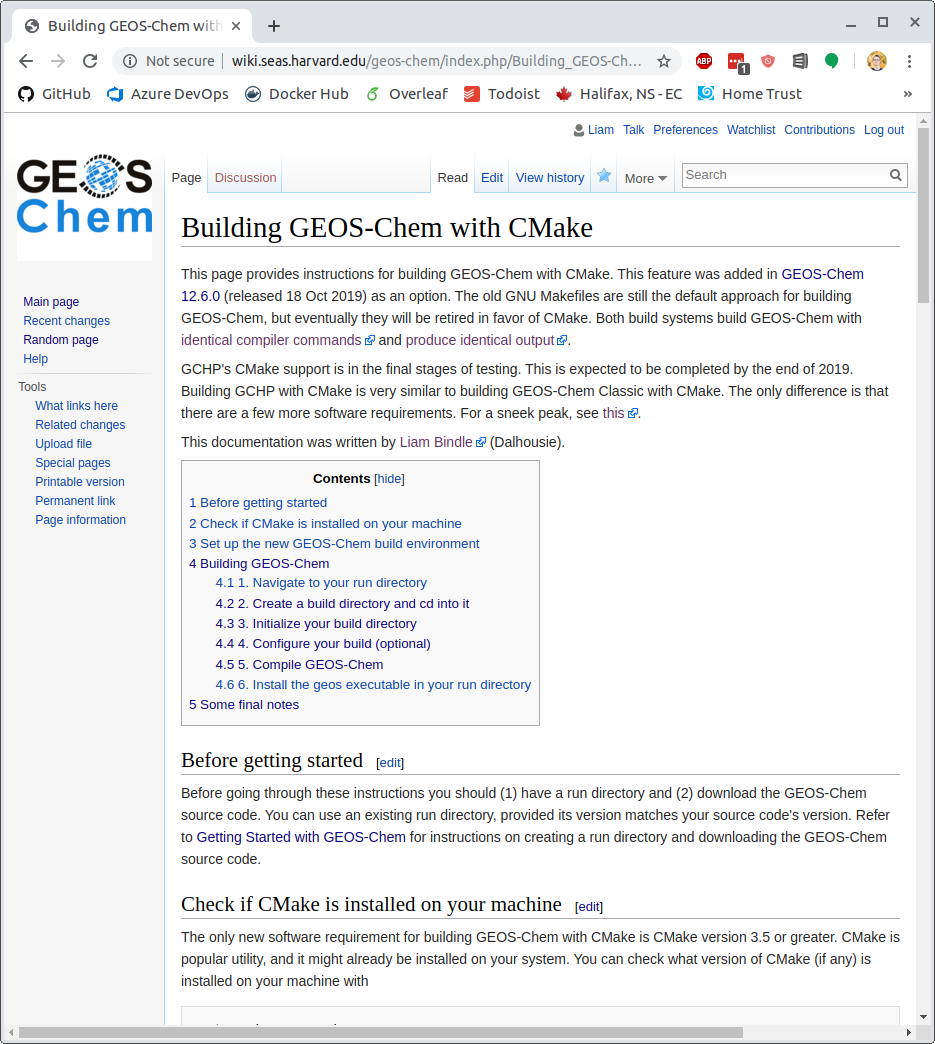
\includegraphics[width=\textwidth]{cmake.png}
    \end{minipage}
\end{frame}

\begin{frame}[fragile]{Improving GCHP quality assurance: CI/CD support}
    \begin{center}
        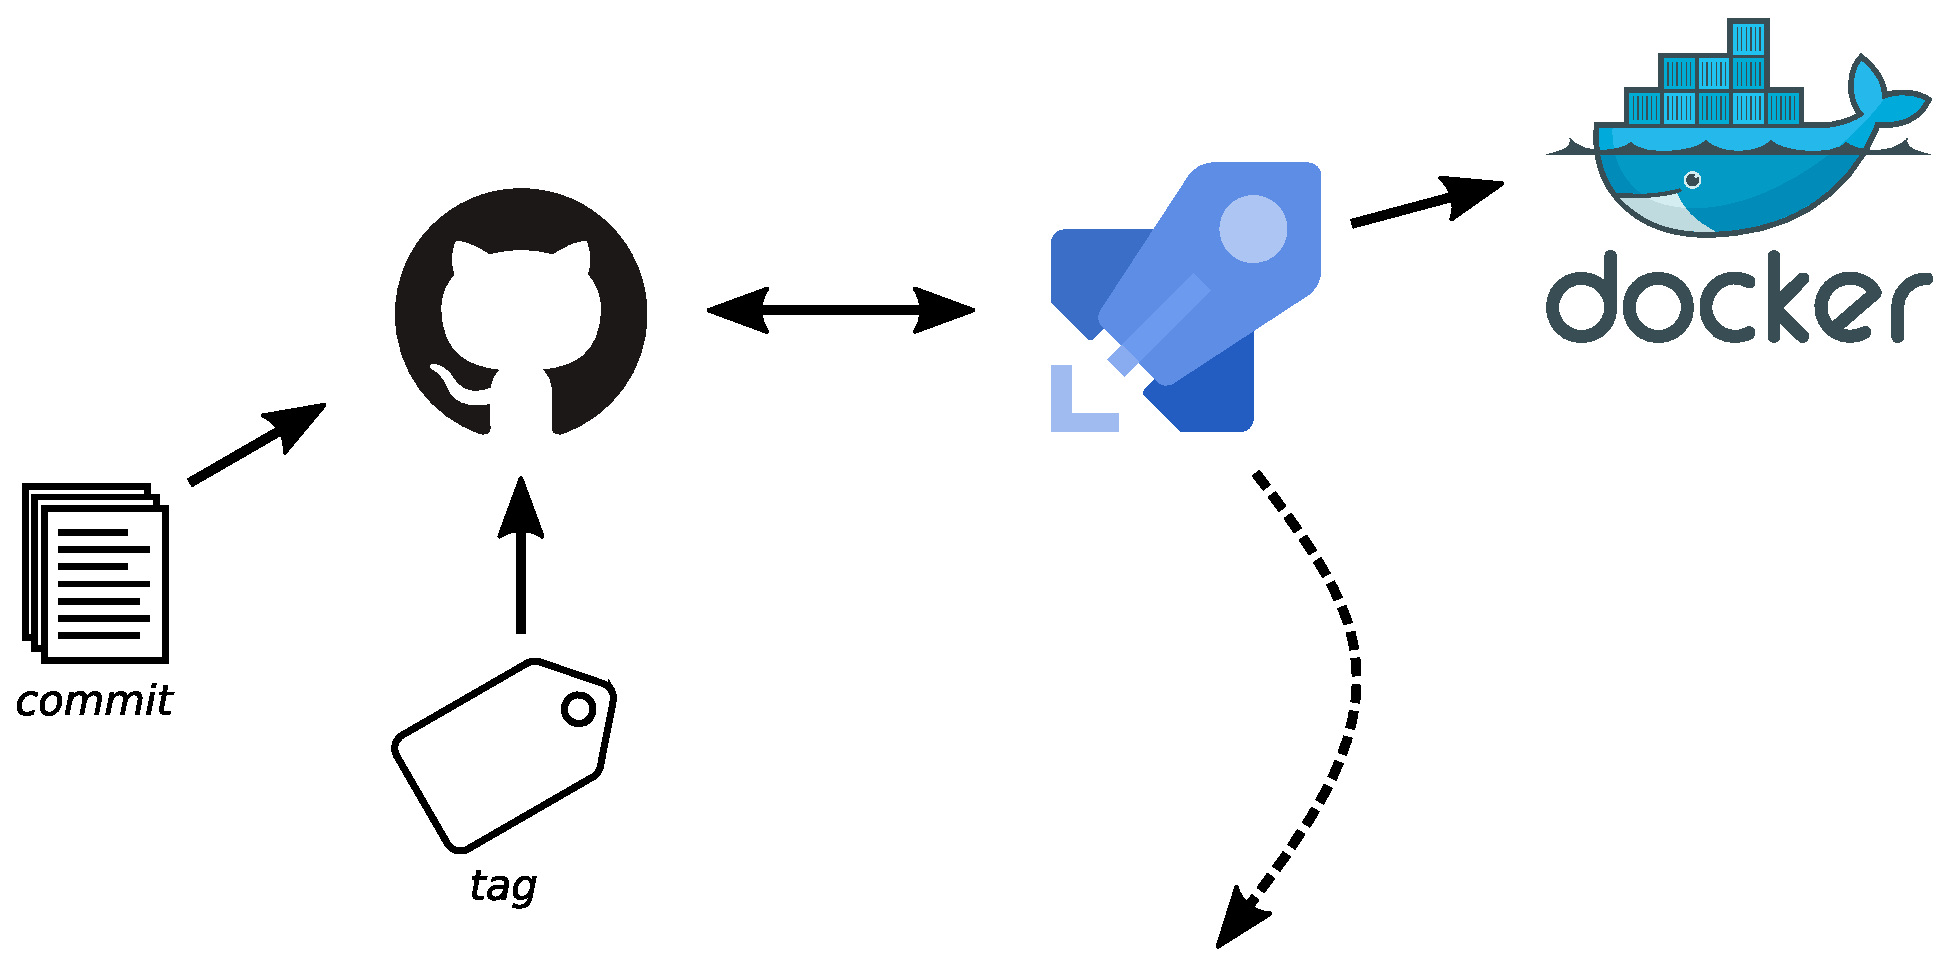
\includegraphics[height=0.3\textheight]{pipeline.eps}
        \vfill
        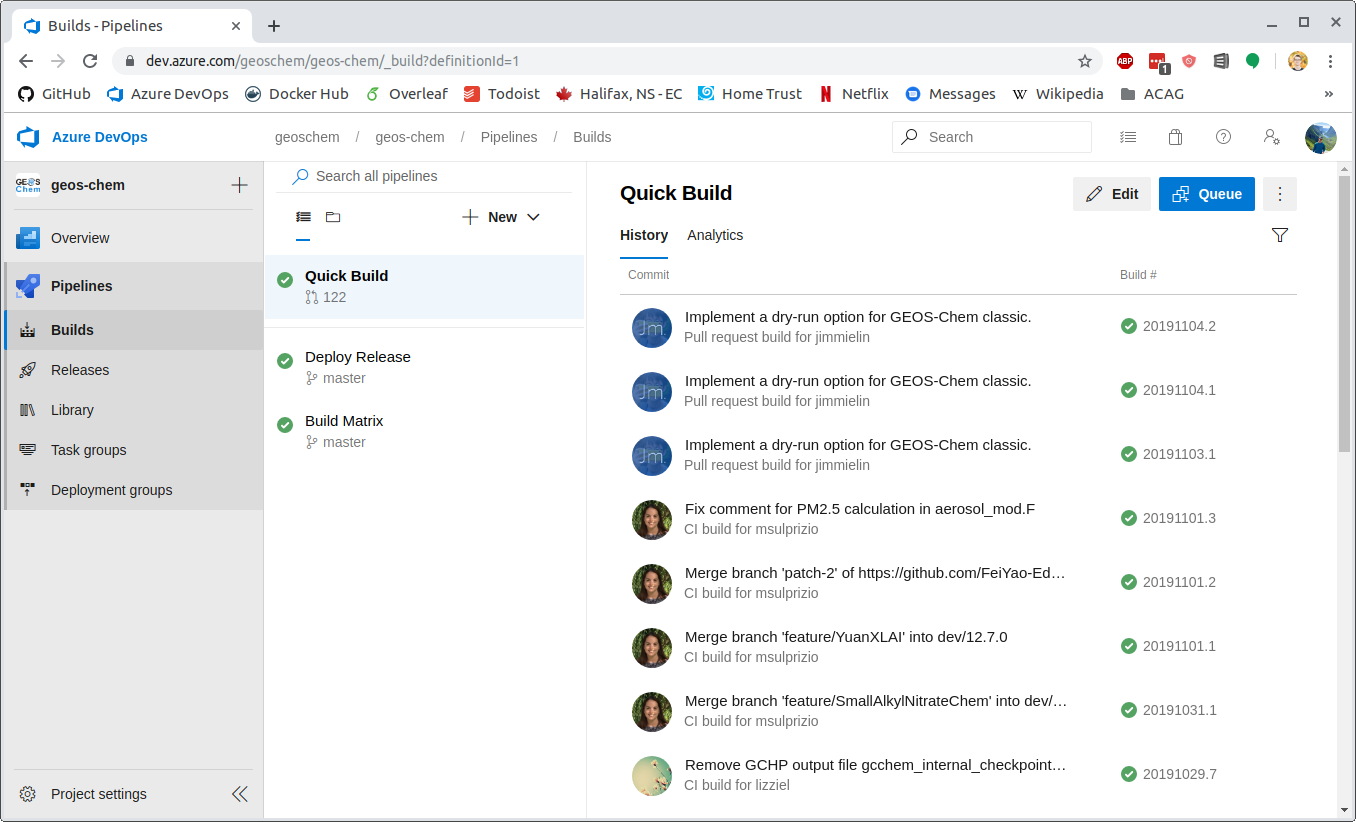
\includegraphics[height=0.5\textheight]{CI.png}
    \end{center}
\end{frame}

\section{GEOS-Chem at high-resolutions}

\begin{frame}[fragile]{How long does GEOS-Chem take to run?}
    \small
    \begin{table}[]
    \begin{tabular}{lcc}
        \hline
        \textbf{Grid} & \multicolumn{2}{c}{\textbf{What does 2-weeks of compute time get you?}} \\ 
        (global) & 1 node & 10 nodes \\ 
        \hline
        C24 & 4 years* & --- \\ 
        C48 & 1 year &  10 years \\ 
        C90 & \semitransp[60]{3 months} & 3 years \\ 
        C180 & \semitransp[60]{1 month} & 8 months \\ 
        C360 & \semitransp[60]{6 days} & 2 months \\ 
        \semitransp[60]{C720} & \semitransp[60]{1-2 days} & \semitransp[60]{10-20 days} \\ \hline
        \multicolumn{3}{r}{\fontsize{4}{4}\selectfont\textit{*Based on 32-core timing test by \cite{yantosca_timing_2018}. All other values are extrapolations assuming perfect scaling.}} \\ 
    \end{tabular}
    \end{table}
    
    \pause
    
    Assuming perfect scaling
    $$\text{wall time} \propto \frac{\text{boxes} \times \text{timesteps}}{\text{CPUs}}$$
    
    so \textbf{doubling global horizontal resolution increases wall time by about 4x} (i.e. horizontal grid complexity is $O(n^2)$)    
\end{frame}

\begin{frame}[fragile]{How much resolution do we need?}
    \begin{figure}
        \centering
        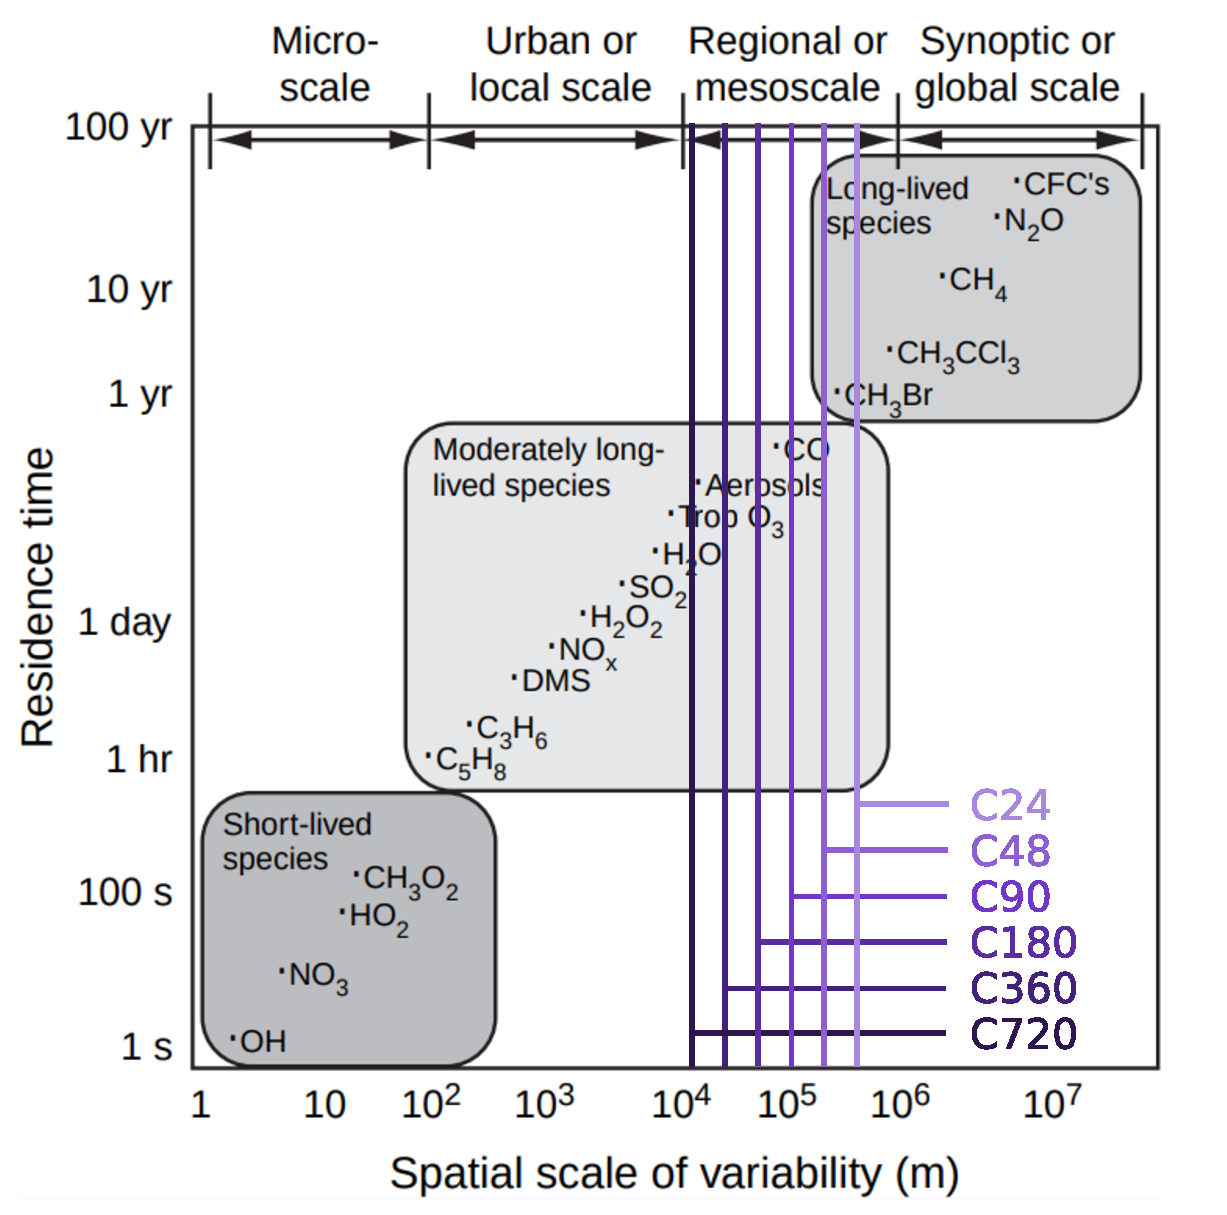
\includegraphics[width=0.6\textwidth]{species-scale.eps}
        \captionsetup{labelformat=empty}
        \caption{Figure from \cite{wallace_atmospheric_2006} overlaid \\ with cube-sphere resolutions.}
    \end{figure}
\end{frame}

\begin{frame}[fragile]{How much resolution do we need?}
    \begin{minipage}[c]{0.5\textwidth}
        \begin{figure}
            \centering
            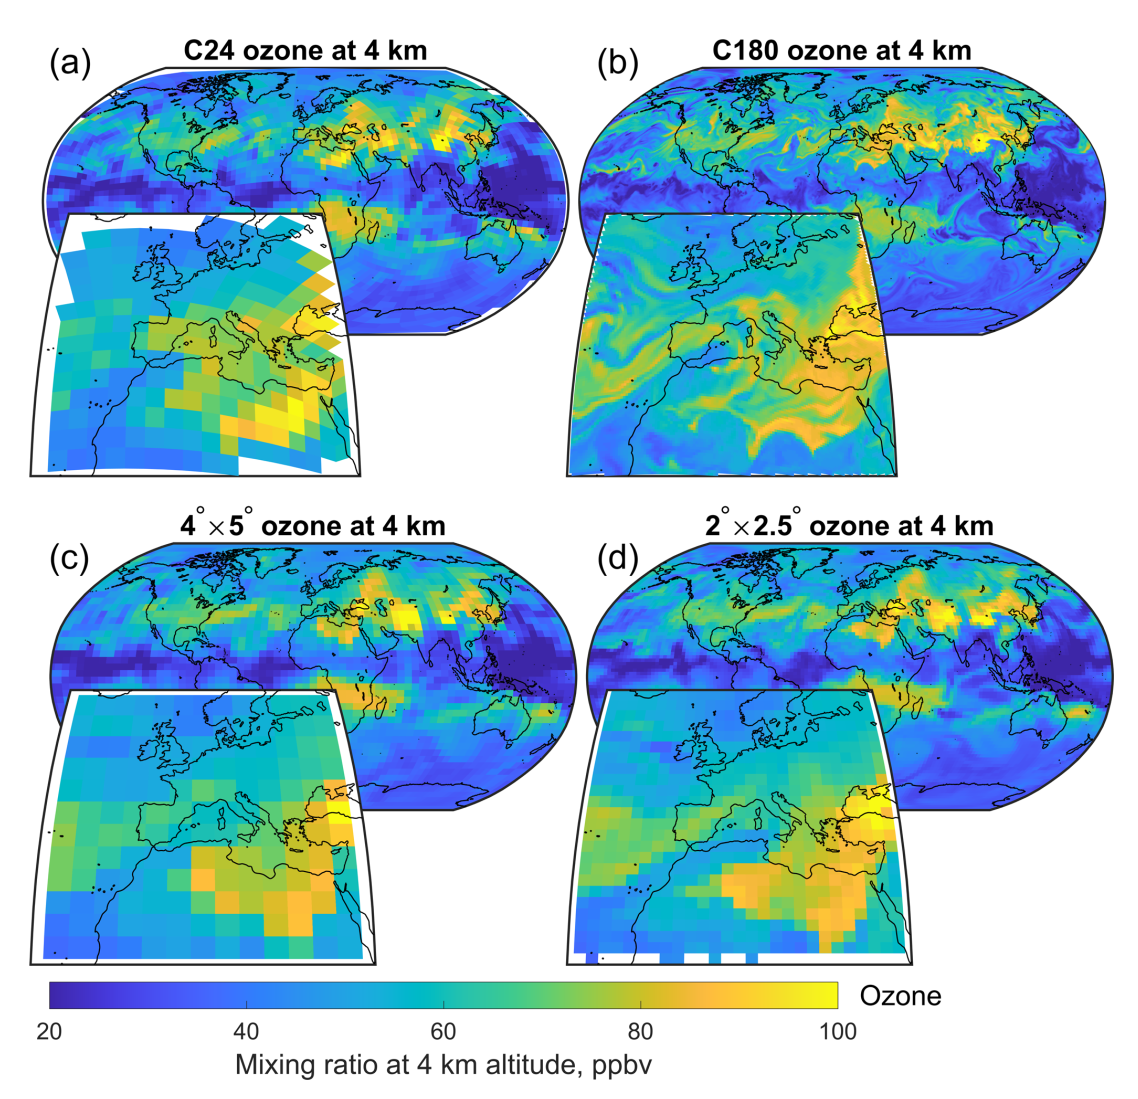
\includegraphics[width=\textwidth]{easthamp.png}
            \captionsetup{labelformat=empty}
            \caption{Figure from \cite{eastham_geos-chem_2018}}
        \end{figure}
    \end{minipage}
    \begin{minipage}[c]{0.49\textwidth}
        \begin{figure}
            \centering
            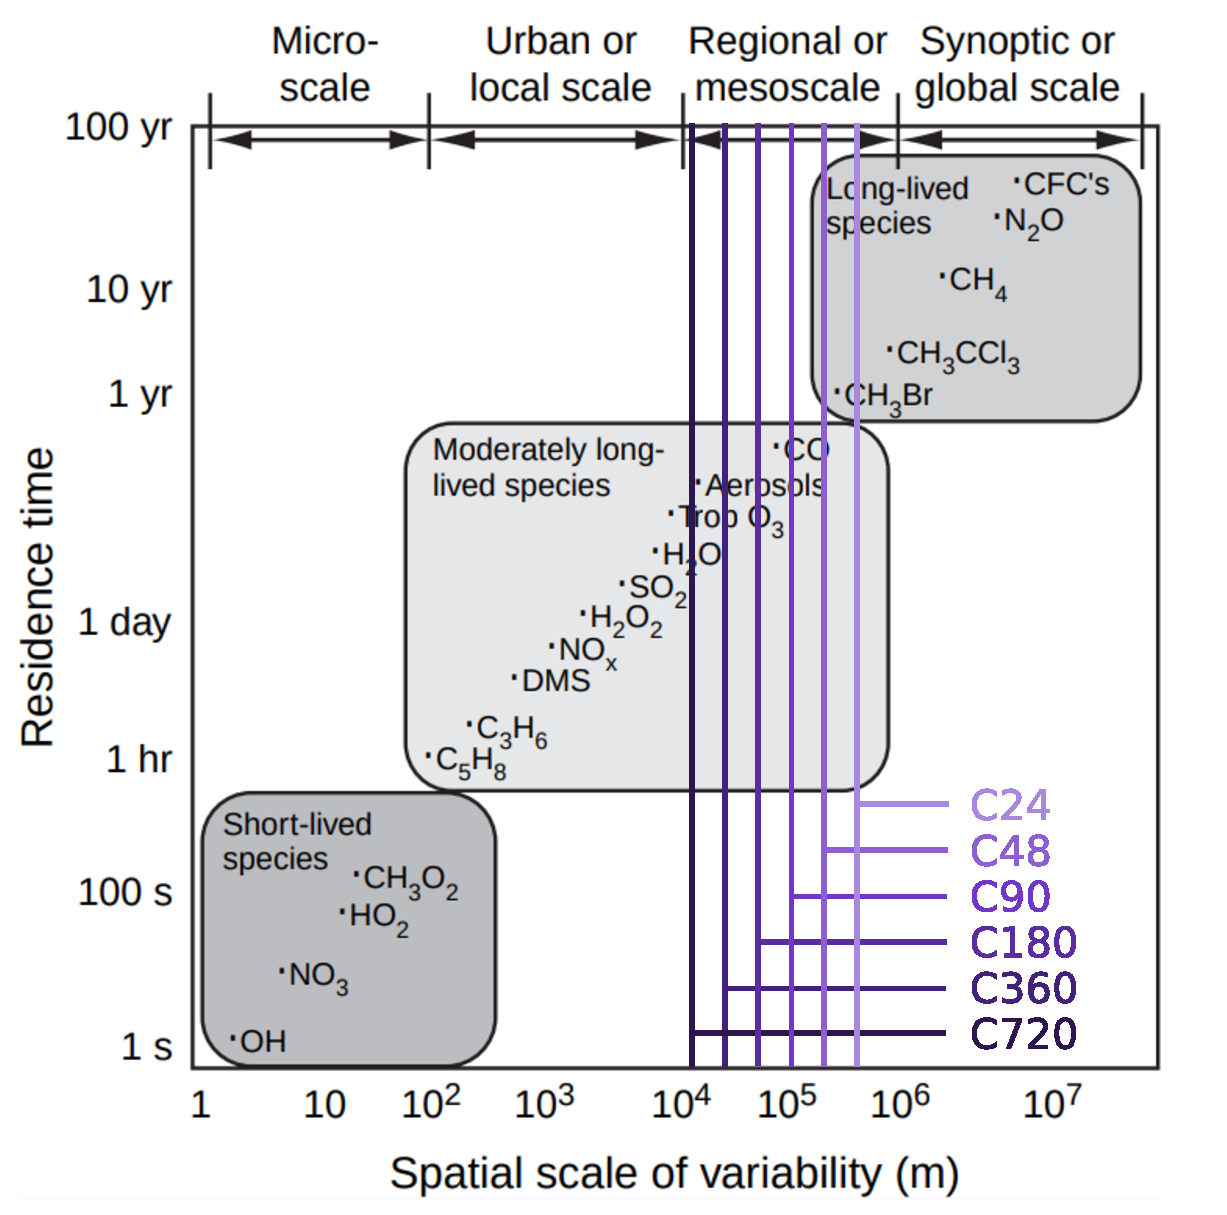
\includegraphics[width=\textwidth]{species-scale.eps}
            \captionsetup{labelformat=empty}
            \caption{Figure from \cite{wallace_atmospheric_2006} overlaid \\ with cube-sphere resolutions.}
        \end{figure}
    \end{minipage}
\end{frame}

\begin{frame}[fragile]{Nested simulations}
    \begin{itemize}
        \item GC Classic has the option to run nested simulations
    \end{itemize}
    
    \footnotesize
    \begin{table}[]
    \begin{tabular}{lccl}
        \hline
        \textbf{Nested Resolution} & \textbf{CS equiv.} &  \textbf{Available Regions} & \textbf{Total wall time} \\ 
        \hline
        0.5$^{\circ}$x0.625$^{\circ}$ & C180e & AS, EU, NA & About 2x longer* \\ 
        0.25$^{\circ}$x0.3125$^{\circ}$ & C360e & CH, EU, NA & About 2-4x longer* \\ 
        \hline
        \multicolumn{4}{r}{\tiny\textit{*Relative to a global $2 \times 2.5$ simulation.}} \\ 
    \end{tabular}
    \end{table}
    \normalsize
    \begin{itemize}
        \item Nested simulations are common
    \end{itemize}
    \vfill
    \begin{itemize}
        \item GCHP doesn't support nested simulations (yet)
        \vspace{0.3cm}
        \item GCHP 13.0.0 will support stretched-grid simulations
    \end{itemize}
\end{frame}

\subsection{Stretched-grid}
\frame{\sectionpage}

\begin{frame}[fragile]{Nested simulation analog for GCHP: stretched-grid support}
    \begin{minipage}[c]{0.5\textwidth}
        \footnotesize
        \begin{itemize}
            \item Transformation that stretches the cube-sphere's boxes
            \item Higher res. on one face, lower res. on the opposite face
            \item No computational expense
            \item 3 parameters
            \begin{itemize}
                \footnotesize
                \item Stretching-factor
                \item Target latitude
                \item Target longitude
            \end{itemize}
            \item e.g. C180 with stretching factor of 2
            \begin{itemize}
                \footnotesize
                \item C360e on target face
                \item C90e opposite target face
                \item Computational expense of C180
            \end{itemize}
        \end{itemize}
    \end{minipage}
    \begin{minipage}[c]{0.48\textwidth}
        \begin{center}
            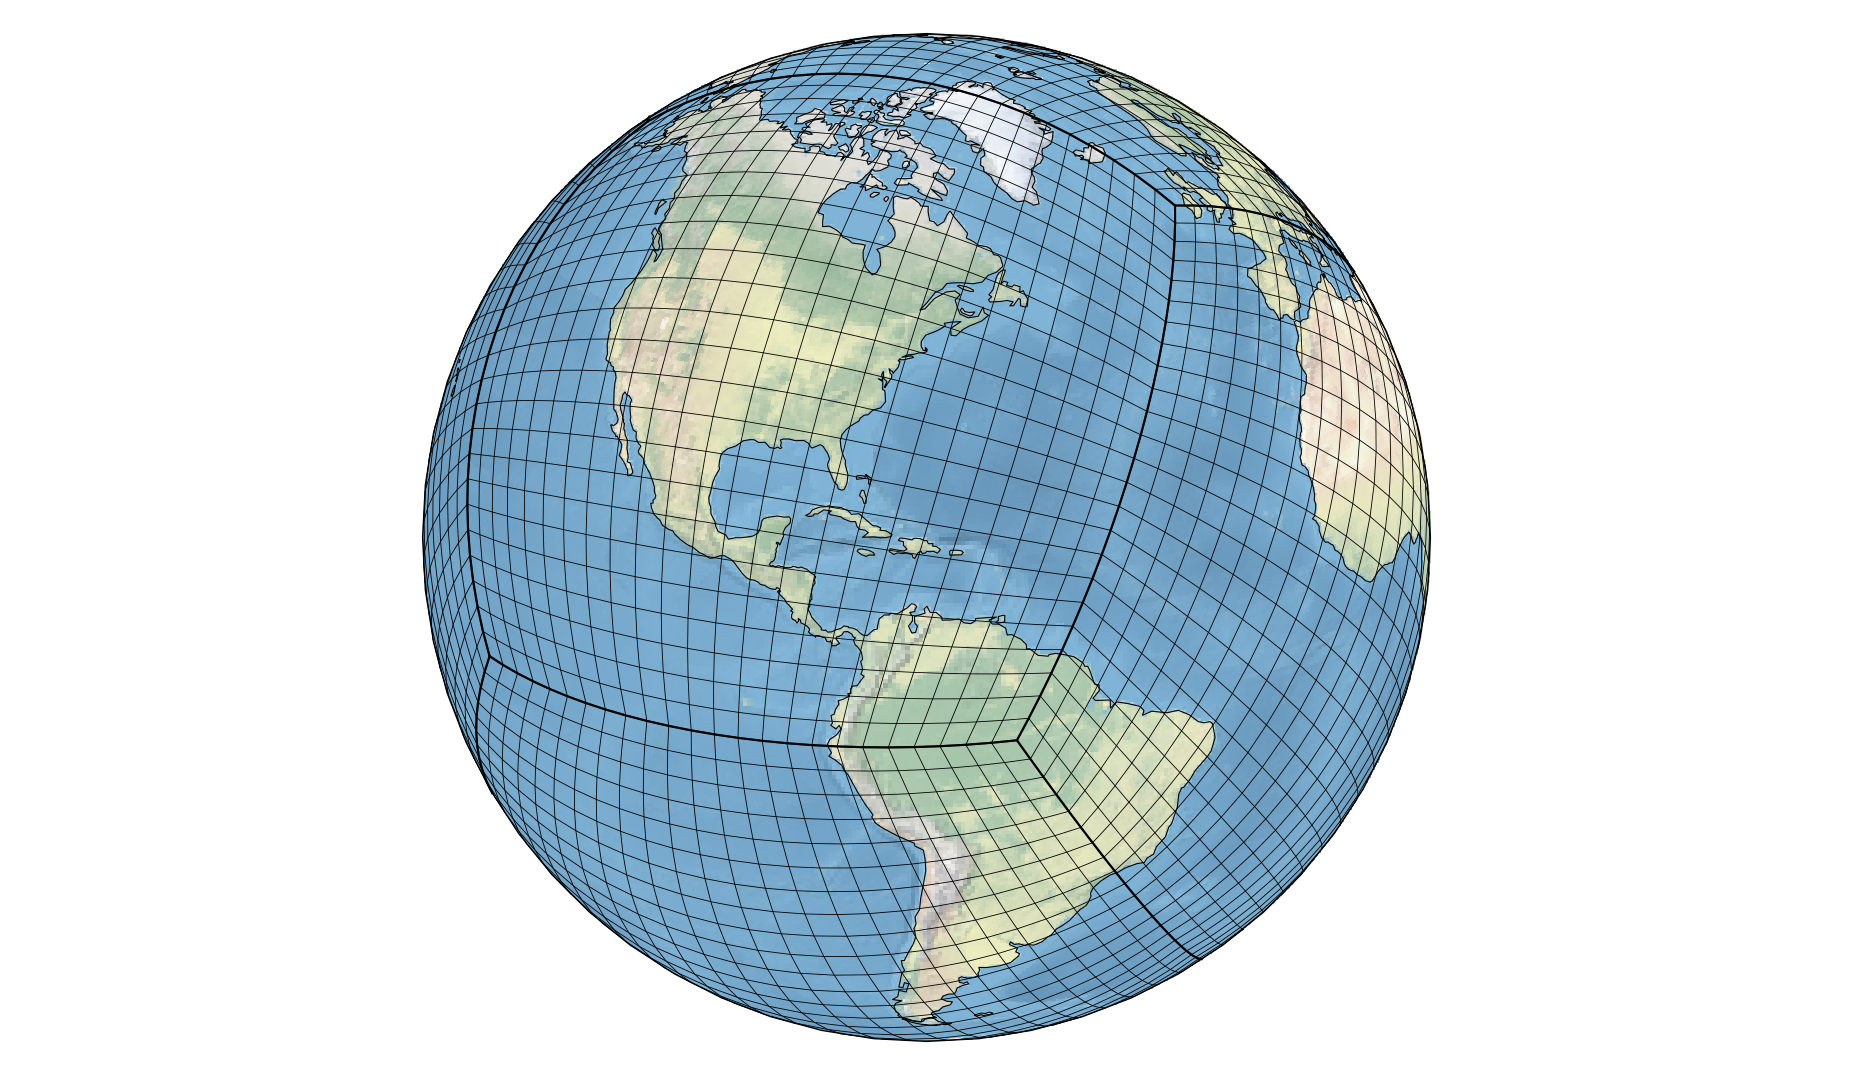
\includegraphics[height=0.3\textheight]{scs_1.png}
        \end{center}
        \begin{center}
            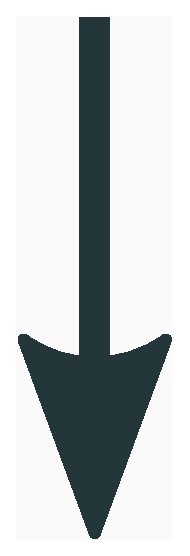
\includegraphics[height=0.05\textheight]{downarrow.eps}
        \end{center}
        \begin{center}
            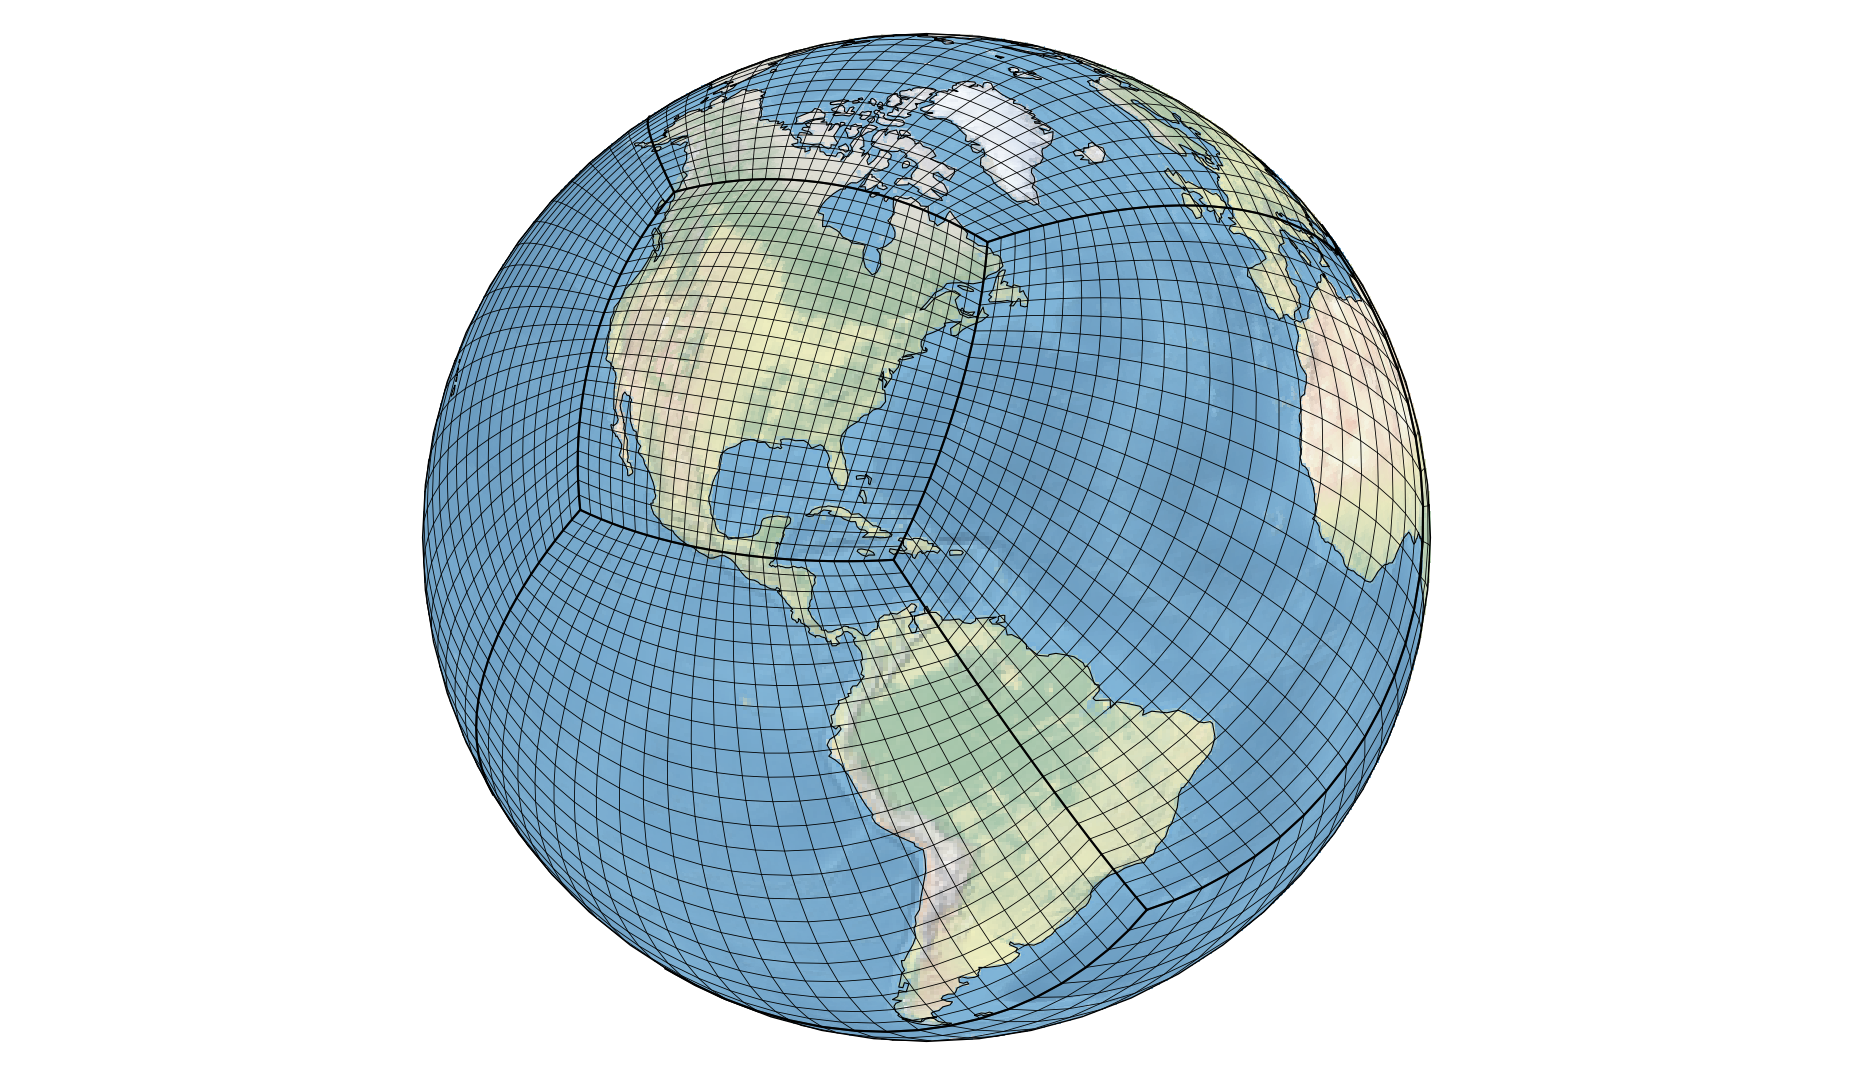
\includegraphics[height=0.3\textheight]{scs_2.png}
        \end{center}
    \end{minipage}
\end{frame}

\begin{frame}{Next steps: investigating grid stretching}
    \vspace{0.4cm}
    \footnotesize
    \textbf{Planned Simulations}
    \tiny
    \begin{table}[]
    \begin{tabular}{cccccc}
        \hline
        \textbf{Simulation \#} & \textbf{Best} & \textbf{Worst} &  \textbf{Actual} & \textbf{SF} & \textbf{C24e runs} \\ 
        \hline
        H.1. & C24 & C24 & C24 & 1 & 1  \\ 
        H.2. & C36 & C36 & C36 & 1 & 2  \\ 
        H.3. & C48 & C48 & C48 & 1 & 4  \\ 
        H.4. & C72 & C48 & C60 & 1.2 & 6  \\ 
        H.5. & C90 & C48 & C66 & 1.36 & 8  \\ 
        H.6. & C135 & C48 & C84 & 1.61 & 12  \\ 
        H.7. & C180 & C48 & C96 & 1.88 & 16  \\ 
        H.8. & C270 & C48 & C114 & 2.37 & 23  \\ 
        H.9. & C360 & C48 & C132 & 2.72 & 30  \\ 
        \hline
         &  &  & & \textbf{Total} & \textbf{102}*  \\ 
         \multicolumn{6}{r}{\fontsize{3}{3}\selectfont\textit{Assuming 3.5 days for a 1-year C24 sim and perfect scaling, suite of simulations would take about 1 core year (about 4.7 w/o SF).}} \\
    \end{tabular}
    \end{table}
    
    \tiny
    \begin{table}[]
    \begin{tabular}{cccccc}
        \hline
        \textbf{Simulation \#} & \textbf{Best} & \textbf{Worst} &  \textbf{Actual} & \textbf{SF} & \textbf{C24e runs} \\ 
        \hline
        ``Truth'' & C360 & C360 & C360 & 1 & 225  \\ 
        E.1. & C540 & C48 & C162 & 3.3 & 46  \\ 
        E.2. & C720 & C48 & C192 & 3.75 & 64  \\ 
        \hline
         &  &  & & \textbf{Total} & \textbf{335}  \\ 
    \end{tabular}
    \end{table}
    
    \footnotesize
    \textbf{Questions}
    \begin{itemize}
        \item How large can the stretching factor be?
        \item How does horizontal grid resolution affect simulated surface level PM$_{2.5}$ and tropospheric O$_3$ and NO$_x$?
    \end{itemize}
\end{frame}

\begin{frame}{Next steps: RIS cluster status}
    \begin{itemize}
        \item I can connect to \texttt{compute1-client-1.ris.wustl.edu}
        \vspace{0.4cm}
        \item Globus transfer from Compute Canada is almost finished
        \vspace{0.4cm}
        \item Good progress on containers for ACAG
        \begin{itemize}
            \footnotesize
            \vspace{0.1cm}
            \item Interactive container
            \vspace{0.1cm}
            \item Official release containers
            \vspace{0.1cm}
            \item Experiment pipeline
        \end{itemize}
        \vspace{0.4cm}
        \item Probably a couple weeks to being operational
        \vspace{0.4cm}
        \item Hoping to start a $2^\circ \times 2.5^\circ$ spin up this week
    \end{itemize}
\end{frame}

\begin{frame}{}
  \centering \Large
  \emph{Thank you!}
\end{frame}

\begin{frame}[allowframebreaks]{References}
    \nocite{geos-chem_developers_narrative_2019}
    \nocite{geos-chem_developers_boundary_2019}
    \tiny
  \bibliography{bib}
  
  %\bibliographystyle{abbrv}

\end{frame}

\end{document}
